\documentclass[dvipdfmx]{jsarticle}
\setcounter{section}{3}
\setcounter{subsection}{1}
\usepackage{xr}
\externaldocument{3.3.1}
\usepackage{amsmath,amsfonts,amssymb,array,comment,mathtools,url,docmute}
\usepackage{longtable,booktabs,dcolumn,tabularx,mathtools,multirow,colortbl,xcolor}
\usepackage[dvipdfmx]{graphics}
\usepackage{bmpsize}
\usepackage{amsthm}
\usepackage{enumitem}
\setlistdepth{20}
\renewlist{itemize}{itemize}{20}
\setlist[itemize]{label=•}
\renewlist{enumerate}{enumerate}{20}
\setlist[enumerate]{label=\arabic*.}
\setcounter{MaxMatrixCols}{20}
\setcounter{tocdepth}{3}
\newcommand{\rotin}{\text{\rotatebox[origin=c]{90}{$\in $}}}
\renewcommand{\thesection}{第\arabic{section}部}
\renewcommand{\thesubsection}{\arabic{section}.\arabic{subsection}}
\renewcommand{\thesubsubsection}{\arabic{section}.\arabic{subsection}.\arabic{subsubsection}}
\everymath{\displaystyle}
\allowdisplaybreaks[4]
\usepackage{vtable}
\theoremstyle{definition}
\newtheorem{thm}{定理}[subsection]
\newtheorem*{thm*}{定理}
\newtheorem{dfn}{定義}[subsection]
\newtheorem*{dfn*}{定義}
\newtheorem{axs}[dfn]{公理}
\newtheorem*{axs*}{公理}
\renewcommand{\headfont}{\bfseries}
\makeatletter
  \renewcommand{\section}{%
    \@startsection{section}{1}{\z@}%
    {\Cvs}{\Cvs}%
    {\normalfont\huge\headfont\raggedright}}
\makeatother
\makeatletter
  \renewcommand{\subsection}{%
    \@startsection{subsection}{2}{\z@}%
    {0.5\Cvs}{0.5\Cvs}%
    {\normalfont\LARGE\headfont\raggedright}}
\makeatother
\makeatletter
  \renewcommand{\subsubsection}{%
    \@startsection{subsubsection}{3}{\z@}%
    {0.4\Cvs}{0.4\Cvs}%
    {\normalfont\Large\headfont\raggedright}}
\makeatother
\makeatletter
\renewenvironment{proof}[1][\proofname]{\par
  \pushQED{\qed}%
  \normalfont \topsep6\p@\@plus6\p@\relax
  \trivlist
  \item\relax
  {
  #1\@addpunct{.}}\hspace\labelsep\ignorespaces
}{%
  \popQED\endtrivlist\@endpefalse
}
\makeatother
\renewcommand{\proofname}{\textbf{証明}}
\usepackage{tikz,graphics}
\usepackage[dvipdfmx]{hyperref}
\usepackage{pxjahyper}
\hypersetup{
 setpagesize=false,
 bookmarks=true,
 bookmarksdepth=tocdepth,
 bookmarksnumbered=true,
 colorlinks=false,
 pdftitle={},
 pdfsubject={},
 pdfauthor={},
 pdfkeywords={}}
\begin{document}
%\hypertarget{ux74b0ux6e96ux540cux578bux5199ux50cf}{%
\subsection{環準同型写像}%\label{ux74b0ux6e96ux540cux578bux5199ux50cf}}
%\hypertarget{ideal}{%
\subsubsection{ideal}%\label{ideal}}
\begin{axs}[idealの公理]
環$R$が与えられたとき、これの空集合でない部分集合$J$が次のことを満たすとき、その集合$J$をその環$R$の左idealという。
\begin{itemize}
\item
  $\forall a,b \in J$に対し、$a + b \in J$が成り立つ。
\item
  $\forall a \in J\forall r \in R$に対し、$ra \in J$が成り立つ。
\end{itemize}
同様に、環$R$が与えられたとき、これの空集合でない部分集合$J$が次のことを満たすとき、その集合$J$をその環$R$の右idealという。
\begin{itemize}
\item
  $\forall a,b \in J$に対し、$a + b \in J$が成り立つ。
\item
  $\forall a \in J\forall r \in R$に対し、$ar \in J$が成り立つ。
\end{itemize}
さらに、環$R$の左idealであるかつ、右idealであるものをその環$R$のideal、両側idealという。
\end{axs}\par
例えば、集合$2\mathbb{Z}$はその集合$\mathbb{Z}$のidealである。
\begin{thm}\label{3.3.2.1}
環$R$の左ideal$J$が与えられたとき、組$(J, + )$は可換群をなし、これの単位元を$1_{(J, + )}$とおくと、次のことを満たす。
\begin{align*}
1_{(J, + )} = 0,\ \ a^{- 1} = - a
\end{align*}
同様に環$R$の右ideal$J$が与えられたとき、組$(J, + )$は可換群をなし、これの単位元を$1_{(J, + )}$とおくと、次のことを満たす。
\begin{align*}
1_{(J, + )} = 0,\ \ a^{- 1} = - a
\end{align*}
\end{thm}
\begin{proof}
環$R$の左ideal$J$が与えられたとき、$\forall a \in J$に対し、$- 1 \in R$より$( - 1)a = - a \in J$が成り立つ。したがって、$a - a = 0 \in J$が成り立つことになるので、次のようになる。
\begin{align*}
(a + b) + c &= a + (b + c)\\
0 + a &= a + 0 = a\\
a - a &= - a + a = 0\\
a + b &= b + a
\end{align*}
したがって、組$(J, + )$は可換群をなし、これの単位元を$1_{(J, + )}$とおくと、次のことを満たす。
\begin{align*}
1_{(J, + )} = 0,\ \ a^{- 1} = - a
\end{align*}
右idealについても同様にして、示される。
\end{proof}
\begin{thm}\label{3.3.2.2}
可換環$R$の左ideal$J$が与えられたとき、これはidealでもある。同様に、可換環$R$の右ideal$J$が与えられたとき、これはidealでもある。
\end{thm}
\begin{proof}
可換環$R$の左ideal$J$が与えられたとき、この部分集合$J$は定義より次のことを満たす。
\begin{itemize}
\item
  $\forall a,b \in J$に対し、$a + b \in J$が成り立つ。
\item
  $\forall a \in J\forall r \in R$に対し、$ra \in J$が成り立つ。
\end{itemize}
ここで、その環$R$は乗法について可換的なので、$ra = ar$が成り立つ。したがって、次のことを満たす。
\begin{itemize}
\item
  $\forall a,b \in J$に対し、$a + b \in J$が成り立つ。
\item
  $\forall a \in J\forall r \in R$に対し、$ra \in J$が成り立つ。
\end{itemize}
よって、その左ideal$J$はその環$R$の右idealでもあるので、その左idealはその環$R$のidealでもある。その環$R$の右idealについても同様にして示される。
\end{proof}
\begin{thm}\label{3.3.2.3}
添数集合$\varLambda_{n}$によって添数づけられた環$R$の元の族$\left\{ a_{i} \right\}_{i \in \varLambda_{n}}$が与えられたとき、その環$R$の元の族$\left\{ r_{i} \right\}_{i \in \varLambda_{n}}$を用いて$\sum_{i \in \varLambda_{n}} {r_{i}a_{i}}$の形で書かれるその環$R$の元全体の集合、即ち、集合$\sum_{i \in \varLambda_{n}} {Ra_{i}}$はその環$R$の左idealとなる。同様に、集合$\sum_{i \in \varLambda_{n}} {a_{i}R}$もその環$R$の右idealである。
\end{thm}
\begin{dfn}
そのような集合たち$\sum_{i \in \varLambda_{n}} {Ra_{i}}$、$\sum_{i \in \varLambda_{n}} {a_{i}R}$をそれぞれその元の族$\left\{ a_{i} \right\}_{i \in \varLambda_{n}}$から生成されたその環$R$の左ideal、右idealという。特に、$n = 1$のとき、その元$a_{1}$から生成されたその環$R$の単項左ideal、単項右idealという。特に、単項左idealであるかつ、単項右idealであるものを単項idealといい、ある整域$R$のidealが全て単項idealであるようなその整域$R$を単項ideal整域という。
\end{dfn}
\begin{dfn}
零元$0$から生成された環$R$の単項左ideal$R0$は明らかに単項右idealでもあり集合$0R$を零idealという。
\end{dfn}
\begin{proof}
添数集合$\varLambda_{n}$によって添数づけられた環$R$の元の族$\left\{ a_{i} \right\}_{i \in \varLambda_{n}}$が与えられたとき、その環$R$の元の族$\left\{ r_{i} \right\}_{i \in \varLambda_{n}}$を用いて$\sum_{i \in \varLambda_{n}} {r_{i}a_{i}}$の形で書かれるその環$R$の元全体の集合、即ち、集合$\sum_{i \in \varLambda_{n}} {Ra_{i}}$について、$\forall\sum_{i \in \varLambda_{n}} {r_{i}a_{i}} \in \sum_{i \in \varLambda_{n}} {Ra_{i}}$に対し、加法と乗法の定義より$\sum_{i \in \varLambda_{n}} {r_{i}a_{i}} \in R$が成り立つので、その集合$\sum_{i \in \varLambda_{n}} {Ra_{i}}$はその環$R$の部分集合である。さらに、$\forall\sum_{i \in \varLambda_{n}} {r_{i}a_{i}},\ \ \sum_{i \in \varLambda_{n}} {s_{i}a_{i}} \in \sum_{i \in \varLambda_{n}} {Ra_{i}}$に対し、次のようになり、
\begin{align*}
\sum_{i \in \varLambda_{n}} {r_{i}a_{i}} + \sum_{i \in \varLambda_{n}} {s_{i}a_{i}} &= \sum_{i \in \varLambda_{n}} \left( r_{i}a_{i} + s_{i}a_{i} \right)\\
&= \sum_{i \in \varLambda_{n}} {\left( r_{i} + s_{i} \right)a_{i}}
\end{align*}
$\forall i \in \varLambda_{n}$に対し、$r_{i} + s_{i} \in R$が成り立つので、$\sum_{i \in \varLambda_{n}} {r_{i}a_{i}} + \sum_{i \in \varLambda_{n}} {s_{i}a_{i}} \in \sum_{i \in \varLambda_{n}} {Ra_{i}}$が成り立つかつ、$\forall r \in R\forall\sum_{i \in \varLambda_{n}} {r_{i}a_{i}} \in \sum_{i \in \varLambda_{n}} {Ra_{i}}$に対し、次のようになり、
\begin{align*}
r\sum_{i \in \varLambda_{n}} {r_{i}a_{i}} &= \sum_{i \in \varLambda_{n}} {rr_{i}a_{i}}\\
&= \sum_{i \in \varLambda_{n}} {\left( rr_{i} \right)a_{i}}
\end{align*}
$\forall i \in \varLambda_{n}$に対し、$rr_{i} \in R$が成り立つので、$r\sum_{i \in \varLambda_{n}} {r_{i}a_{i}} \in \sum_{i \in \varLambda_{n}} {Ra_{i}}$が成り立つ。以上より、その集合$\sum_{i \in \varLambda_{n}} {Ra_{i}}$はその環$R$の左idealとなる。同様にして、集合$\sum_{i \in \varLambda_{n}} {a_{i}R}$もその環$R$の右idealであることが示される。
\end{proof}
\begin{thm}\label{3.3.2.4}
零環でない環$R$が斜体であるならそのときに限り、その環$R$は零ideal$0R$とその環$R$自身以外に左idealをもたない。\par
同様に、環$R$が斜体であるならそのときに限り、その環$R$は零ideal$R0$とその環$R$自身以外に右idealをもたない\footnote{ただ、その環$R$は零ideal$R0$とその環$R$自身以外にidealをもたないなら、その環$R$は斜体であるということは成り立たないということにお気をつけて…。}。
\end{thm}
\begin{proof}
零環でない環$R$が斜体であるとする。その環$R$の任意の左ideal$J$が与えられたとき、これが零idealでないなら、$a \neq 0$なるその左ideal$J$の元$a$が存在し、その環$R$は斜体なので、元$a^{-1}$がその環$R$に存在することになり、したがって、$a^{-1}a = 1 \in J$が成り立つ。したがって、$\forall a \in R$に対し、$a1 = a \in J$が成り立つことになり、よって、$R = J$が成り立つ。ゆえに、その環$R$は零ideal$0R$とその環$R$自身以外に左idealをもたない。\par
逆に、零環でない環$R$は零ideal$0R$とその環$R$自身以外に左idealをもたないとしよう。このとき、$\forall a \in R$に対し、$a \neq 0$が成り立つなら、これによって生成されたその環$R$の単項左ideal$Ra$は零idealでないので、$Ra = R$が成り立つことになる。したがって、$\forall a' \in R$に対し、$a'a \neq 1$が成り立つなら、$Ra \subset R$が成り立つので、対偶律より$a'a = 1$なるその環$R$の元$a'$が存在する。これが$0$であるなら、$1 = 0$となり矛盾しているので、$a' \neq 0$が成り立つ。同様にして、$a''a' = 1$なる元$a''$がその環$R$に存在することになり、したがって、次のようになる。
\begin{align*}
a'' &= a''1\\
&= a''\left( a'a \right)\\
&= \left( a''a' \right)a\\
&= 1a = a
\end{align*}
これにより、$a'a = aa' = 1$なる元$a'$がその環$R$に存在することになり、したがって、$\forall a \in R$に対し、$a \neq 0$が成り立つなら、これは可逆元であるから、その環$R$は斜体である。
\end{proof}
\begin{thm}\label{3.3.2.5}
環$R$の左idealたち$I$、$J$が与えられたとき、集合たち$I \cap J$、$I + J$もその環$R$の左idealである。\par
同様に、環$R$の右idealたち$I$、$J$が与えられたとき、集合たち$I \cap J$、$I + J$もその環$R$の右idealである。
\end{thm}
\begin{proof}
環$R$の左idealたち$I$、$J$が与えられたとき、集合$I \cap J$はもちろんその環$R$の部分集合であり、$\forall a,b \in I \cap J$に対し、$a,b \in I$かつ$a,b \in J$が成り立つので、$a + b \in I$かつ$a + b \in J$が成り立ち、したがって、$a + b \in I \cap J$が成り立つ。$\forall a \in I \cap J$に対し、$a \in I$かつ$a \in J_{2}$が成り立つので、$\forall r \in R$に対し、$ra \in I$かつ$ra \in J$が成り立ち、したがって、$ra \in I \cap J$が成り立つ。\par
$\forall a \in I\forall b \in J$に対し、$a + b \in I + J$が成り立つ。ここで、$a,b \in R$が成り立つので、$a + b \in R$が成り立ち、したがって、その集合$I + J$はその環$R$の部分集合である。このとき、$\forall a,b \in I\forall c,d \in J$に対し、$a + b \in I$かつ$c + d \in J$が成り立つので、$(a + c) + (b + d) = (a + b) + (c + d) \in I + J$が成り立つ。さらに、$\forall a \in I\forall b \in J\forall r \in R$に対し、$ra \in I$かつ$rb \in J$が成り立つので、$r(a + b) = ra + rb \in I + J$が成り立つ。\par
よって、環$R$の左idealたち$I$、$J$が与えられたとき、集合たち$I \cap J$、$I + J$もその環$R$の左idealである。\par
同様にして、環$R$の右idealたち$I$、$J$が与えられたとき、集合たち$I \cap J$、$I + J$もその環$R$の右idealであることが示される。
\end{proof}
%\hypertarget{ux5546ux74b0}{%
\subsubsection{商環}%\label{ux5546ux74b0}}
\begin{dfn}
環$R$とこれの1つのideal$J$を考え$a,b \in R$なる元々$a$、$b$について次のことを定義しよう。このようなことを元たち$a$、$b$がそのideal$J$を法として合同であるという。
\begin{align*}
a \equiv b\ \mathrm{mod}J \Leftrightarrow b - a \in J
\end{align*}
これは群論でいう可換群$(R, + )$の部分群$(J, + )$を法として合同であるという概念と一致する。ゆえに、次の定理\ref{3.3.2.6}、定理\ref{3.3.2.7}、定理\ref{3.3.2.8}が成り立つ。なお、より一般的な証明は群論の書籍などに参照されたい\footnote{たとえば、雪江明彦「群論入門」、松坂和夫「代数系入門」などが挙げられます。}。
\end{dfn}
\begin{thm}\label{3.3.2.6}
環$R$のideal$J$が与えられたとき、$J + J = J$が成り立つ。
\end{thm}
\begin{proof}
環$R$のideal$J$が与えられたとき、$\forall a + b \in J + J$に対し、$a,b \in J$が成り立つので、$a + b \in J$も成り立つ。一方で、$\forall a \in J$に対し、組$(J, + )$は単位元$0$、元$a$の逆元$- a$の可換群をなすので、$- a \in J$が成り立つ。したがって、$a - a = 0 \in J$が成り立ち、したがって、$a = 0 + a$が成り立つので、$a \in J + J$も成り立つ。以上より、$J + J = J$が得られる。
\end{proof}
\begin{thm}\label{3.3.2.7}
環$R$のideal$J$が与えられたとき、関係$\equiv \ \mathrm{mod}J $はその環$R$における同値関係である。
\end{thm}
\begin{proof}
環$R$のideal$J$が与えられたとき、$\forall a,b,c \in R$に対し、組$(J, + )$は単位元$0$、元$a$の逆元$- a$の可換群をなすので、次のようになる。
\begin{align*}
0 \in R &\Rightarrow 0 \in J\\
&\Leftrightarrow a - a \in J\\
&\Leftrightarrow a \equiv a\ \mathrm{mod}J \\
a \equiv b\ \mathrm{mod}J &\Leftrightarrow b - a \in J\\
&\Leftrightarrow - (b - a) = a - b \in J\\
&\Leftrightarrow b \equiv a\ \mathrm{mod}J \\
a \equiv b\ \mathrm{mod}J \land b \equiv c\ \mathrm{mod}J &\Leftrightarrow b - a \in J \land c - b \in J\\
&\Rightarrow (b - a) + (c - b) = c - a \in J\\
&\Leftrightarrow a \equiv c\ \mathrm{mod}J 
\end{align*}
\end{proof}
\begin{thm}\label{3.3.2.8}
環$R$のideal$J$が与えられたとき、同値関係$\equiv \ \mathrm{mod}J $によるその環$R$の元$a$の同値類$C_{\equiv \ \mathrm{mod}J }(a)$は集合$a + J$に等しい。
\end{thm}
\begin{dfn}
この集合$a + J$をそのideal$J$を法とする元$a$の剰余類という。
\end{dfn}
\begin{proof}
環$R$のideal$J$が与えられたとき、同値関係$\equiv \ \mathrm{mod}J $によるその環$R$の元$a$の同値類$C_{\equiv \ \mathrm{mod}J }(a)$について、次のようなり、
\begin{align*}
x \in C_{\equiv \ \mathrm{mod}J }(a) &\Leftrightarrow a \equiv x\ \mathrm{mod}J \\
&\Leftrightarrow x - a \in J
\end{align*}
ここで、$y = x - a$とすると、次式が成り立ち、
\begin{align*}
x &= 0 + x = (a - a) + x\\
&= a + (x - a)\\
&= a + y
\end{align*}
明らかに$y \in J$かつ$a + y \in R$が成り立つので、次式が成り立ち、
\begin{align*}
a + y \in C_{\equiv \ \mathrm{mod}J }(a) &\Leftrightarrow a + y \in R \land a \equiv a + y\ \mathrm{mod}J \\
&\Leftrightarrow a + y \in R \land (a + y) - a \in J\\
&\Leftrightarrow a + y \in R \land y \in J\\
&\Leftrightarrow a + y \in \left\{ a + y \in R \middle| y \in J \right\} = a + J
\end{align*}
したがって、次のようになる。
\begin{align*}
C_{\equiv \ \mathrm{mod}J }(a) &= \left\{ a + y \in R \middle| y \in J \right\}\\
&= a + J
\end{align*}
\end{proof}
\begin{dfn}
環$R$のideal$J$が与えられたとき、そのideal$J$を法とする剰余類たち$a + J$全体の集合を${R}/{J}$と書く、即ち、次式のようにおく。
\begin{align*}
{R}/{J} = \left\{ a + J \middle| a \in R \right\}
\end{align*}
\end{dfn}
\begin{thm}[idealを法とする剰余類分解]\label{3.3.2.7s}
環$R$のideal$J$が与えられたとき、次式が成り立つ。
\begin{align*}
R=\bigsqcup {R/J}
\end{align*}\par
この定理をidealを法とする剰余類分解という。
\end{thm}
\begin{proof}
環$R$のideal$J$が与えられたとき、定理\ref{3.3.2.7}よりその関係$\equiv \ \mathrm{mod}J$はその集合$R$における同値関係であるので、その関係$\equiv\ \mathrm{mod}J$による類別が次のようになる。
\begin{align*}
R=\bigsqcup {R}/{\equiv\ \mathrm{mod}J}=\bigsqcup {R/J}_l
\end{align*}
\end{proof}
\begin{thm}\label{3.3.2.9}
その組$\left( {R}/{J}, + \right)$は可換群をなす。このとき、その可換群$\left( {R}/{J}, + \right)$上での単位元は$0 + J = J$、その可換群$\left( {R}/{J}, + \right)$の任意の元$a + J$の逆元は$- a + J$となる。
\end{thm}
\begin{proof}
環$R$のideal$J$が与えられたとき、そのideal$J$を法とする剰余類たち$a + J$全体の集合${R}/{J}$において、$\forall a,b,c \in R$に対し、次のようになるかつ、
\begin{align*}
(a + J + b + J) + c + J &= (a + b + c) + (J + J + J)\\
&= a + J + (b + J + c + J)
\end{align*}
次のようになるかつ、
\begin{align*}
(0 + J) + (a + J) &= (0 + a) + (J + J) = a + J\\
(a + J) + (0 + J) &= (a + 0) + (J + J) = a + J
\end{align*}
次のようになるかつ、
\begin{align*}
(a + J) + ( - a + J) &= (a - a) + (J + J) = 0 + J = J\\
( - a + J) + (a + J) &= ( - a + a) + (J + J) = 0 + J = J
\end{align*}
次のようになるので、
\begin{align*}
(a + J) + (b + J) = (b + J) + (a + J)
\end{align*}
よって、その組$\left( {R}/{J}, + \right)$は可換群をなす。このとき、その可換群$\left( {R}/{J}, + \right)$上での単位元は$0 + J = J$、その可換群$\left( {R}/{J}, + \right)$の任意の元$a + J$の逆元は$- a + J$となる。
\end{proof}
\begin{thm}\label{3.3.2.10}
環$R$のideal$J$が与えられたとき、$a \equiv b\ \mathrm{mod}J $かつ$c \equiv d\ \mathrm{mod}J $が成り立つなら、$ac \equiv bd\ \mathrm{mod}J $が成り立つ。
\end{thm}
\begin{proof}
環$R$のideal$J$が与えられたとき、$a \equiv b\ \mathrm{mod}J $かつ$c \equiv d\ \mathrm{mod}J $が成り立つなら、$u = b - a$、$v = d - c$とおかれると、$u,v \in J$が成り立つので、したがって、次のようになる。
\begin{align*}
ac &= (b - u)(d - v)\\
&= bd + b( - v) + ( - u)d + ( - u)( - v)\\
&= bd + ( - b)v + u( - d) + uv
\end{align*}
ここで、$( - b)v,u( - d),uv \in J$が成り立つので、$( - b)v + u( - d) + uv \in J$が成り立つ。ゆえに、$ac - bd \in J$が成り立つので、$ac \equiv bd\ \mathrm{mod}J $が成り立つ。
\end{proof}
\begin{thm}\label{3.3.2.11}
環$R$のideal$J$が与えられたとき、$a + J = b + J$かつ$c + J = d + J$が成り立つなら、$ac + J = bd + J$が成り立つ。
\end{thm}
\begin{proof}
環$R$のideal$J$が与えられたとき、$a + J = b + J$かつ$c + J = d + J$が成り立つなら、、$a \equiv b\ \mathrm{mod}J $かつ$c \equiv d\ \mathrm{mod}J $が成り立つ。ここで、定理\ref{3.3.2.10}より$ac \equiv bd\ \mathrm{mod}J $が成り立つことになる。よって、$ac + J = bd + J$が成り立つ。
\end{proof}
\begin{thm}\label{3.3.2.12}
環$R$のideal$J$を法とする剰余類たち$a + J$全体の集合${R}/{J}$は次式のように加法と乗法が定義されれば、
\begin{align*}
+ &:{R}/{J} \times {R}/{J} \rightarrow {R}/{J};(a + J,b + J) \mapsto (a + b) + J\\
\cdot &:{R}/{J} \times {R}/{J} \rightarrow {R}/{J};(a + J,b + J) \mapsto ab + J
\end{align*}
環をなし、このとき、零元、単位元はそれぞれ$J$、$1 + J$となる。
\end{thm}
\begin{dfn}
この環${R}/{J}$をその環$R$のそのideal$J$による商環、剰余環という。
\end{dfn}
\begin{proof}
環$R$のideal$J$を法とする剰余類たち$a + J$全体の集合${R}/{J}$は次式のように加法と乗法が定義されれば、
\begin{align*}
+ &:{R}/{J} \times {R}/{J} \rightarrow {R}/{J};(a + J,b + J) \mapsto (a + b) + J\\
\cdot &:{R}/{J} \times {R}/{J} \rightarrow {R}/{J};(a + J,b + J) \mapsto ab + J
\end{align*}
定理\ref{3.3.2.9}よりその組$\left( {R}/{J}, + \right)$は可換群をなし、このとき、その可換群$\left( {R}/{J}, + \right)$上での単位元は$0 + J = J$、その可換群$\left( {R}/{J}, + \right)$の任意の元$a + J$の逆元は$- a + J$となる。さらに、$\forall a + J,b + J,c + J \in {R}/{J}$に対し、次のようになるので、
\begin{align*}
\left( (a + J)(b + J) \right)(c + J) &= (ab + J)(c + J)\\
&= (ab)c + J\\
&= a(bc) + J\\
&= (a + J)(bc + J)\\
&= (a + J)\left( (b + J)(c + J) \right)\\
(a + J)(1 + J) &= a1 + J\\
&= a + J\\
(1 + J)(a + J) &= 1a + J\\
&= a + J\\
(a + J)\left( (b + J) + (c + J) \right) &= (a + J)\left( (b + c) + J \right)\\
&= a(b + c) + J\\
&= (ab + ac) + J\\
&= (ab + J) + (ac + J)\\
&= (a + J)(b + J) + (a + J)(c + J)\\
\left( (a + J) + (b + J) \right)(c + J) &= \left( (a + b) + J \right)(c + J)\\
&= (a + b)c + J\\
&= (ac + bc) + J\\
&= (ac + J) + (bc + J)\\
&= (a + J)(c + J) + (b + J)(c + J)
\end{align*}
環$R$のideal$J$を法とする剰余類たち$a + J$全体の集合${R}/{J}$は環をなし、このとき、零元、単位元はそれぞれ$J$、$1 + J$となる。
\end{proof}
%\hypertarget{ux74b0ux6e96ux540cux578bux5199ux50cf-1}{%
\subsubsection{環準同型写像}%\label{ux74b0ux6e96ux540cux578bux5199ux50cf-1}}
\begin{dfn}
2つの環々$R$、$S$が与えられこれらの零元をそれぞれ$0_{R}$、$0_{S}$、単位元をそれぞれ$1_{R}$、$1_{S}$とするとき、次のことを満たすような写像$f:R \rightarrow S$をその環$R$からその環$S$への環準同型写像という。
\begin{itemize}
\item
  $\forall a,b \in R$に対し、$f(a + b) = f(a) + f(b)$が成り立つ。
\item
  $\forall a,b \in R$に対し、$f(ab) = f(a)f(b)$が成り立つ。
\item
  $f\left( 1_{R} \right) = 1_{S}$が成り立つ。
\end{itemize}
\end{dfn}
\begin{thm}\label{3.3.2.13}
2つの環々$R$、$S$、その環$R$からその環$S$への環準同型写像$f$が与えられこれらの2つの環々$R$、$S$の零元をそれぞれ$0_{R}$、$0_{S}$、単位元をそれぞれ$1_{R}$、$1_{S}$とするとき、次のことが成り立つ。
\begin{itemize}
\item
  $f\left( 0_{R} \right) = 0_{S}$が成り立つ。
\item
  $\forall a \in R$に対し、$f( - a) = - f(a)$が成り立つ。
\end{itemize}
\end{thm}
\begin{proof}
2つのの環々$R$、$S$、その環$R$からその環$S$への環準同型写像$f$が与えられこれらの2つの環々$R$、$S$の零元をそれぞれ$0_{R}$、$0_{S}$、単位元をそれぞれ$1_{R}$、$1_{S}$とするとき、次のようになる。
\begin{align*}
f\left( 0_{R} \right) &= f\left( 0_{R} \right) + 0_{S}\\
&= f\left( 0_{R} \right) + f\left( 0_{R} \right) - f\left( 0_{R} \right)\\
&= f\left( 0_{R} + 0_{R} \right) - f\left( 0_{R} \right)\\
&= f\left( 0_{R} \right) - f\left( 0_{R} \right) = 0_{S}
\end{align*}\par
また、$\forall a \in R$に対し、次のようになる。
\begin{align*}
f( - a) &= f( - a) + 0_{S}\\
&= f( - a) + f(a) - f(a)\\
&= f( - a + a) - f(a)\\
&= f\left( 0_{1} \right) - f(a)\\
&= 0_{S} - f(a)\\
&= - f(a)
\end{align*}
\end{proof}
\begin{thm}\label{3.3.2.14}
3つの環々$R$、$S$、$T$、その環$R$からその環$S$への環準同型写像$f$、その環$S$からその環$T$への環準同型写像$g$が与えられこれらの3つの環々$R$、$S$、$T$の単位元をそれぞれ$1_{R}$、$1_{S}$、$1_{T}$とするとき、その合成写像$g \circ f$も環準同型写像である。
\end{thm}
\begin{proof}
3つの環々$R$、$S$、$T$、その環$R$からその環$S$への環準同型写像$f$、その環$S$からその環$T$への環準同型写像$g$が与えられこれらの3つの環々$R$、$S$、$T$の単位元をそれぞれ$1_{R}$、$1_{S}$、$1_{T}$とするとき、$\forall a,b \in R$に対し、次のようになる。
\begin{align*}
g \circ f(a + b) &= g\left( f(a + b) \right)\\
&= g\left( f(a) + f(b) \right)\\
&= g\left( f(a) \right) + g\left( f(b) \right)\\
&= g \circ f(a) + g \circ f(b)\\
g \circ f(ab) &= g\left( f(ab) \right)\\
&= g\left( f(a)f(b) \right)\\
&= g\left( f(a) \right)g\left( f(b) \right)\\
&= g \circ f(a)g \circ f(b)\\
g \circ f\left( 1_{R} \right) &= g\left( f\left( 1_{R} \right) \right)\\
&= g\left( 1_{S} \right) = 1_{T}
\end{align*}
\end{proof}
\begin{dfn}
環準同型写像のうち、全射であるもの、単射であるもの、全単射であるものをそれぞれ全射環準同型写像、単射環準同型写像、環同型写像という。
\end{dfn}
\begin{thm}\label{3.3.2.15}
2つの環々$R$、$S$、その環$R$からその環$S$への環同型写像$f$が与えられこれらの2つの環々$R$、$S$の単位元をそれぞれ$1_{R}$、$1_{S}$とするとき、その写像$f$の逆写像$f^{- 1}$も環同型写像である。
\end{thm}
\begin{proof}
2つの環々$R$、$S$、その環$R$からその環$S$への環同型写像$f$が与えられこれらの2つの環々$R$、$S$の単位元をそれぞれ$1_{R}$、$1_{S}$とするとき、$\forall a,b \in S$に対し、次のようになる。
\begin{align*}
f^{- 1}(a + b) &= f^{- 1}\left( f \circ f^{- 1}(a) + f \circ f^{- 1}(b) \right)\\
&= f^{- 1}\left( f\left( f^{- 1}(a) \right) + f\left( f^{- 1}(b) \right) \right)\\
&= f^{- 1}\left( f\left( f^{- 1}(a) + f^{- 1}(b) \right) \right)\\
&= f^{- 1} \circ f\left( f^{- 1}(a) + f^{- 1}(b) \right)\\
&= f^{- 1}(a) + f^{- 1}(b)\\
f^{- 1}(ab) &= f^{- 1}\left( f \circ f^{- 1}(a)f \circ f^{- 1}(b) \right)\\
&= f^{- 1}\left( f\left( f^{- 1}(a) \right)f\left( f^{- 1}(b) \right) \right)\\
&= f^{- 1}\left( f\left( f^{- 1}(a)f^{- 1}(b) \right) \right)\\
&= f^{- 1} \circ f\left( f^{- 1}(a)f^{- 1}(b) \right)\\
&= f^{- 1}(a)f^{- 1}(b)\\
f^{- 1}\left( 1_{S} \right) &= 1_{R}
\end{align*}
\end{proof}
\begin{dfn}
2つの環々$R$、$S$は、その環$R$からその環$S$への環準同型写像$f:R\overset{\sim}{\rightarrow}S$が存在するとき、環同型であるといい$R \cong S$と書く。
\end{dfn}
\begin{thm}\label{3.3.2.16}
次のことが成り立つ、即ち、その関係$\cong$は同値関係である。
\begin{itemize}
\item
  $R \cong R$が成り立つ。
\item
  $R \cong S$が成り立つなら、$S \cong R$も成り立つ。
\item
  $R \cong S$かつ$S \cong T$が成り立つなら、$R \cong T$も成り立つ。
\end{itemize}
\end{thm}
\begin{proof}
環同型な3つの環々$R$、$S$、$T$が与えられこれらの単位元をそれぞれ$1_{R}$、$1_{S}$、$1_{T}$とする。\par
その環$R$の恒等写像$I_{R}$を考えると、$\forall a,b \in R$に対し、次のようになり、
\begin{align*}
I_{R}(a + b) &= a + b = I_{R}(a) + I_{R}(b)\\
I_{R}(ab) &= ab = I_{R}(a)I_{R}(b)\\
I_{R}\left( 1_{R} \right) &= 1_{R}
\end{align*}
恒等写像の逆写像はもとのその恒等写像自身であるので、この写像$I_{R}$は環同型写像である。よって、$R \cong R$が成り立つ。\par
$R \cong S$が成り立つなら、その環$R$からその環$S$への環同型写像$f$が存在し、環同型写像の逆対応は環同型写像であったので、その環$S$からその環$R$への環同型写像が存在し$S \cong R$が成り立つ。\par
$R \cong S$かつ$S \cong T$が成り立つなら、その環$R$からその環$S$への環同型写像$f$が存在するかつ、その環$S$からその環$T$への環同型写像$g$が存在し、ここで、その写像$g \circ f$も環準同型写像であり、さらに、これらの逆写像たち$f^{- 1}$、$g^{- 1}$も環同型写像たちであるので、その合成写像$f^{- 1} \circ g^{- 1}$も環準同型写像である。ここで、次のようになるので、
\begin{align*}
(g \circ f) \circ \left( f^{- 1} \circ g^{- 1} \right) &= g \circ \left( f \circ f^{- 1} \right) \circ g^{- 1}\\
&= g \circ I_{S} \circ g^{- 1}\\
&= g \circ g^{- 1} = I_{T}\\
\left( f^{- 1} \circ g^{- 1} \right) \circ (g \circ f) &= f^{- 1} \circ \left( g^{- 1} \circ g \right) \circ f\\
&= f^{- 1} \circ I_{S} \circ f\\
&= f^{- 1} \circ f = I_{R}
\end{align*}
その写像$f^{- 1} \circ g^{- 1}$はその写像$g \circ f$の逆写像でありその写像$g \circ f$は環同型写像となる。よって、$R \cong T$が成り立つ。
\end{proof}
\begin{thm}\label{3.3.2.17}
2つの環々$R$、$S$の間の環準同型写像$f:R \rightarrow S$の値域$V(f)$はその環$S$の部分環である。
\end{thm}
\begin{proof}
2つの環々$R$、$S$の間の環準同型写像$f:R \rightarrow S$の値域$V(f)$について、これらの環々の単位元をそれぞれ$1_{R}$、$1_{S}$とおくと、$f\left( 1_{R} \right) = 1_{S}$が成り立つのであったので、$1_{S} \in V(f)$が成り立つ。また、$\forall f(a),f(b) \in V(f)$に対し、$a,b \in R$なる元々$a$、$b$が存在し、$f( - a) \in V(f)$で$- f(a) = f( - a)$が成り立つので、$- f(a) \in V(f)$が成り立つ。さらに、$f(a + b) = f(a) + f(b) \in V(f)$が成り立つかつ、$f(ab) = f(a)f(b) \in V(f)$が成り立つので、その値域$V(f)$はその環$S$の部分環である。
\end{proof}
\begin{dfn}
2つの環々$R$、$S$の間の環準同型写像$f:R \rightarrow S$について、この環$S$の零元を$0_{S}$とおくと、$f(a) = 0_{S}$なるその環$R$の元々$a$全体の集合をその写像$f$の核といい、$\ker f$などと書く、即ち、次式のように定められる\footnote{なお、その環$S$が零環でないかぎり、その環$R$の単位元はその核$\ker f$に属しえませんので、$R = \ker f$が成り立つことはありません。}。
\begin{align*}
\ker f = \left\{ a \in R \middle| f(a) = 0_{S} \right\}
\end{align*}
\end{dfn}
\begin{thm}\label{3.3.2.18}
2つの環々$R$、$S$の間の環準同型写像$f:R \rightarrow S$の核$\ker f$はその環$R$のidealである。
\end{thm}
\begin{proof}
2つの環々$R$、$S$の間の環準同型写像$f:R \rightarrow S$の核$\ker f$について、この環$S$の零元を$0_{S}$とおくと、$\forall a,b \in \ker f$に対し、次のようになるので、
\begin{align*}
f(a + b) &= f(a) + f(b)\\
&= 0_{S} + 0_{S} = 0_{S}
\end{align*}
$a + b \in \ker f$が成り立つかつ、$\forall a \in \ker f\forall r \in R$に対し、次のようになるので、
\begin{align*}
f(ra) &= f(r)f(a)\\
&= f(r)0_{S} = 0_{S}
\end{align*}
$ra \in \ker f$が成り立つ。以上より、その核$\ker f$はその環$R$の左idealである。同様にして、その核$\ker f$はその環$R$の右idealであることが示される。
\end{proof}
%\hypertarget{ux81eaux7136ux306aux5168ux5c04ux74b0ux6e96ux540cux578bux5199ux50cf}{%
\subsubsection{自然な全射環準同型写像}%\label{ux81eaux7136ux306aux5168ux5c04ux74b0ux6e96ux540cux578bux5199ux50cf}}
\begin{thm}\label{3.3.2.19}
環$R$のideal$J$が与えられたとき、写像$\varphi:R \rightarrow {R}/{J};a \mapsto a + J$はその環$R$から商環${R}/{J}$への全射準同型写像であり$\ker\varphi = J$が成り立つ。
\end{thm}
\begin{dfn}
このように次式のような写像$\varphi$をその環$R$からその商環${R}/{J}$への自然な全射環準同型写像、標準的環準同型写像という。\
\begin{center}
  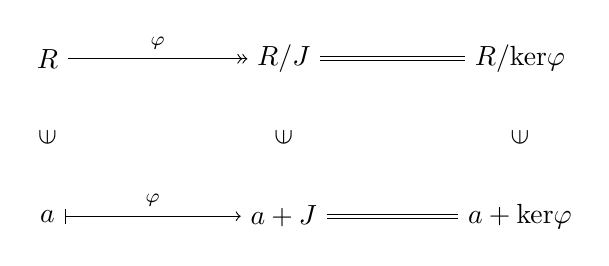
\begin{tikzpicture}[auto]
    \node[rotate=90] (a) at (0, 1) {$\in $};
    \node[rotate=90] (b) at (3, 1) {$\in $};
    \node[rotate=90] (c) at (6, 1) {$\in $};
    \node (a) at (0, 2) {$R$};
    \node (b) at (3, 2) {$R/J$};
    \node (c) at (6, 2) {$R/{\rm ker} \varphi $};
    \draw [->>] (a) to node {$\scriptstyle \varphi $} (b);
    \draw [double distance=1pt] (b) to node {$\scriptstyle $} (c);
    \node (a) at (0, 0) {$a$};
    \node (b) at (3, 0) {$a+J$};
    \node (c) at (6, 0) {$a+{\rm ker} \varphi $};
    \draw [|->] (a) to node {$\scriptstyle \varphi $} (b);
    \draw [double distance=1pt] (b) to node {$\scriptstyle $} (c);
  \end{tikzpicture}
\end{center}
\end{dfn}
\begin{proof}
環$R$のideal$J$が与えられたとき、写像$\varphi:R \rightarrow {R}/{J};a \mapsto a + J$について、$\forall a,b \in R$に対し、次のようになる。
\begin{align*}
\varphi(a + b) &= (a + b) + J\\
&= (a + J) + (b + J)\\
&= \varphi(a) + \varphi(b)\\
\varphi(ab) &= ab + J\\
&= (a + J)(b + J)\\
&= \varphi(a)\varphi(b)\\
\varphi(1) &= 1 + J
\end{align*}
これにより、その写像$\varphi$は環準同型写像である。\par
また、その商環${R}/{J}$の零元は$J$であるので、$\forall a \in \ker\varphi$に対し、次のようになる。
\begin{align*}
\varphi(a) = a + J = J
\end{align*}
ここで、$\forall b \in J$に対し、$b = a + b'$なる元$b'$がそのideal$J$に存在し次のようになるので、
\begin{align*}
a &= a + 0\\
&= a + b' - b'\\
&= b - b' \in J
\end{align*}
$a \in J$が成り立つ。逆に、$\forall a \in J$が成り立つなら、次のようになるので、
\begin{align*}
\varphi(a) &= a + J\\
&= \left\{ a + b \in R \middle| b \in J \right\}\\
&= \left\{ a + b \in R \middle| a + b \in J \right\}\\
&= J
\end{align*}
$a \in \ker\varphi$が成り立つ。以上より、$\ker\varphi = J$が得られる。\par
最後に、$\forall a + J \in {R}/{J}$に対し、商環の定義より明らかに$\varphi(a) = a + J$なるその環$R$の元$a$が存在するので、その写像$\varphi$は全射である。これにより、その写像$\varphi$は全射環準同型写像である。
\end{proof}
%\hypertarget{ux74b0ux6e96ux540cux578bux5b9aux7406}{%
\subsubsection{環準同型定理}%\label{ux74b0ux6e96ux540cux578bux5b9aux7406}}
\begin{thm}\label{3.3.2.20}
2つの環々$R$、$S$の間の環準同型写像$f:R \rightarrow S$が与えられたとき、その環$R$が斜体でそれらの環々$R$、$S$が零環でないなら、その写像$f$は単射環準同型写像である。
\end{thm}
\begin{proof}
2つの環々$R$、$S$の間の環準同型写像$f:R \rightarrow S$が与えられたとき、その環$R$が斜体でそれらの環々$R$、$S$が零環でないなら、その環$R$のidealは定理\ref{3.3.2.4}より零idealかその環$R$自身しかもたないことになる。ここで、その環$S$が零環でないので、その核$\ker f$はその環$R$自身になりえないので、その核$\ker f$は零idealであることになる。このとき、$\forall f(a),f(b) \in V(f)$に対し、$f(a) = f(b)$が成り立つなら、その環$S$の零元を$0_{S}$として次のようになり、
\begin{align*}
f(a) = f(b) &\Leftrightarrow f(a) - f(b) = f(a) + f( - b) = f(a - b) = 0_{S}\\
&\Leftrightarrow a - b \in \ker f\\
&\Leftrightarrow a - b \in R0\\
&\Leftrightarrow a - b = 0\\
&\Leftrightarrow a = b
\end{align*}
その写像$f$は単射である。よって、その環$R$が斜体でそれらの環々$R$、$S$が零環でないなら、その写像$f$は単射環準同型写像である。
\end{proof}
\begin{thm}[環準同型定理]\label{3.3.2.21}
2つの環々$R$、$S$の間の環準同型写像$f:R \rightarrow S$の核$\ker f$が与えられたとき、その環$R$からその商環${R}/{\ker f}$への自然な全射環準同型写像を$\varphi$とおいた次式のような写像$g$は環同型写像である。
\begin{center}
  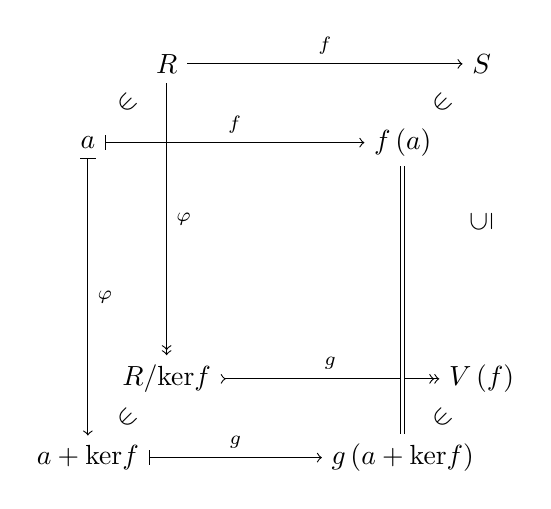
\begin{tikzpicture}[auto]
    \node (a) at (0, 0) {$a+{\rm ker} f$};
    \node (b) at (4, 0) {$g\left( a+{\rm ker} f\right) $};
    \node (c) at (0, 4) {$a$};
    \node (d) at (4, 4) {$f\left( a\right) $};
    \node (e) at (1, 1) {$R/{\rm ker} f$};
    \node (f) at (5, 1) {$V\left( f\right) $};
    \node (g) at (1, 5) {$R$};
    \node (h) at (5, 5) {$S$};
    \node[rotate=45] (i) at (0.5, 0.5) {$\in $};
    \node[rotate=45] (j) at (4.5, 0.5) {$\in $};
    \node[rotate=45] (k) at (0.5, 4.5) {$\in $};
    \node[rotate=45] (l) at (4.5, 4.5) {$\in $};
    \node[rotate=90] (m) at (5, 3) {$\subseteq $};
    \draw [|->] (a) to node {$\scriptstyle g$} (b);
    \draw [>->>] (e) to node {$\scriptstyle g$} (f);
    \draw [|->] (c) to node {$\scriptstyle \varphi $} (a);
    \draw [->>] (g) to node {$\scriptstyle \varphi $} (e);
    \draw [|->] (c) to node {$\scriptstyle f$} (d);
    \draw [->] (g) to node {$\scriptstyle f$} (h);
    \draw [double distance=1pt] (b) to node {$ $} (d);
  \end{tikzpicture} 
\end{center}
これにより、${R}/{\ker f} \cong V(f)$が成り立つ。\par
この定理を環準同型定理という。
\end{thm}
\begin{proof}
2つの環々$R$、$S$の間の環準同型写像$f:R \rightarrow S$の核$\ker f$が与えられたとき、その環$R$からその商環${R}/{\ker f}$への自然な全射環準同型写像を$\varphi$とおいた次式のような写像$g$について、
\begin{center}
  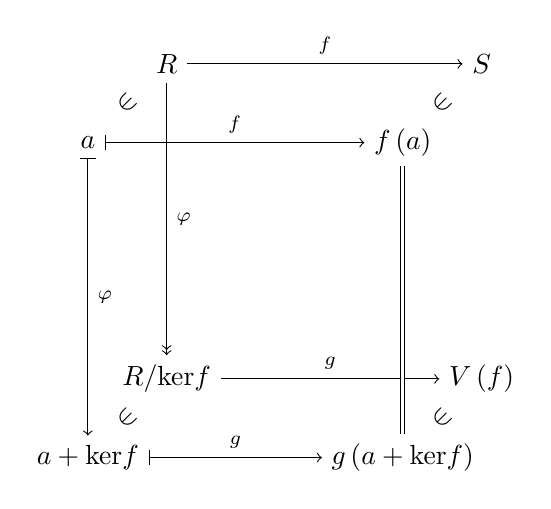
\begin{tikzpicture}[auto]
    \node (a) at (0, 0) {$a+{\rm ker} f$};
    \node (b) at (4, 0) {$g\left( a+{\rm ker} f\right) $};
    \node (c) at (0, 4) {$a$};
    \node (d) at (4, 4) {$f\left( a\right) $};
    \node (e) at (1, 1) {$R/{\rm ker} f$};
    \node (f) at (5, 1) {$V\left( f\right) $};
    \node (g) at (1, 5) {$R$};
    \node (h) at (5, 5) {$S$};
    \node[rotate=45] (i) at (0.5, 0.5) {$\in $};
    \node[rotate=45] (j) at (4.5, 0.5) {$\in $};
    \node[rotate=45] (k) at (0.5, 4.5) {$\in $};
    \node[rotate=45] (l) at (4.5, 4.5) {$\in $};
    \draw [|->] (a) to node {$\scriptstyle g$} (b);
    \draw [->] (e) to node {$\scriptstyle g$} (f);
    \draw [|->] (c) to node {$\scriptstyle \varphi $} (a);
    \draw [->>] (g) to node {$\scriptstyle \varphi $} (e);
    \draw [|->] (c) to node {$\scriptstyle f$} (d);
    \draw [->] (g) to node {$\scriptstyle f$} (h);
    \draw [double distance=1pt] (b) to node {$ $} (d);
  \end{tikzpicture}
\end{center}
この環$R$の単位元を$1_{R}$、この環$S$の零元を$0_{S}$、単位元を$1_{S}$とおくと、その値域の定義より明らかにその写像$g$は全射である。また、$g\left( a + \ker f \right) = g\left( b + \ker f \right)$が成り立つなら、その核$\ker f$はその環$R$のidealであることにより次のようになる。
\begin{align*}
g\left( a + \ker f \right) = g\left( b + \ker f \right) &\Leftrightarrow f(a) = f(b)\\
&\Leftrightarrow f(a) - f(b) = 0_{S}\\
&\Leftrightarrow f(a) + f( - b) = 0_{S}\\
&\Leftrightarrow f(a - b) = 0_{S}\\
&\Leftrightarrow a - b \in \ker f\\
&\Leftrightarrow b - a \in \ker f
\end{align*}
ここで、$b - a \in \ker f$が成り立つなら、$a \equiv b\ \left( \mathrm{mod}{\ker f} \right)$が成り立ち、したがって、$a + \ker f = b + \ker f$が成り立つので、その写像$g$は単射である。以上より、その写像$g$は全単射である。\par
その組$\left( \ker f, + \right)$は群をなすのであったので、$\forall a + \ker f,b + \ker f \in {R}/{\ker f}$に対し、次のようになる。
\begin{align*}
g\left( \left( a + \ker f \right) + \left( b + \ker f \right) \right) &= g\left( (a + b) + \ker f \right)\\
&= f(a + b)\\
&= f(a) + f(b)\\
&= g\left( a + \ker f \right) + g\left( b + \ker f \right)\\
g\left( \left( a + \ker f \right)\left( b + \ker f \right) \right) &= g\left( ab + \ker f \right)\\
&= f(ab)\\
&= f(a)f(b)\\
&= g\left( a + \ker f \right)g\left( b + \ker f \right)\\
g\left( 1_{R} + \ker f \right) &= f\left( 1_{R} \right) = 1_{S}
\end{align*}
これにより、その写像$g$は環準同型写像であり、その写像$g$は全単射だったので、その写像$g$は環同型写像である。\par
これにより、2つのそれらの環々${R}/{\ker f}$、$V(f)$は、その環${R}/{\ker f}$からその環$V(f)$への環同型写像$g:{R}/{\ker f} \rightarrow V(f)$が存在するので、環同型である、即ち、${R}/{\ker f} \cong V(f)$が成り立つ。
\end{proof}
%\hypertarget{ux74b0ux540cux578bux5b9aux7406}{%
\subsubsection{環同型定理}%\label{ux74b0ux540cux578bux5b9aux7406}}
\begin{thm}\label{3.3.2.22}
2つの環々$R$、$S$の間の全射環準同型写像$f:R \twoheadrightarrow S$について、その環$R$の左ideal$I$、右ideal$J$を用いた2つの集合たち$V\left( f|I \right)$、$V\left( f|J \right)$はそれぞれその環$S$の左ideal、右idealである。また、その環$S$の左ideal$I$、右ideal$J$を用いた2つの集合たち$V\left( f^{- 1}|I \right)$、$V\left( f^{- 1}|J \right)$はそれぞれその環$R$の左ideal、右idealである。
\end{thm}
\begin{proof}
2つの環々$R$、$S$の間の全射環準同型写像$f:R \twoheadrightarrow S$について、その環$R$の左ideal$I$が与えられたとき、$\forall f(a),\ f(b) \in V\left( f|I \right)$に対し、定義より$a + b \in I$も成り立つので、次のようになる。
\begin{align*}
f(a) + f(b) = f(a + b) \in V\left( f|I \right)
\end{align*}
$\forall f(a) \in V\left( f|I \right)\forall s \in S$に対し、その写像$f$は全射であるから、$\exists r \in R$に対し、$f(r) = s$が成り立ち、定義より$ra \in I$も成り立つので、次のようになる。
\begin{align*}
sf(a) &= f(r)f(a)\\
&= f(ra)\\
&= f(ra) \in V\left( f|I \right)
\end{align*}
したがって、集合$V\left( f|I \right)$はその環$S$の左idealである。同様にして、その環$R$の右ideal$J$が与えられたとき、集合$V\left( f|J \right)$はその環$S$の右idealであることが示される。\par
また、その環$S$の左ideal$I$が与えられたとき、環準同型写像の定義と左idealの定義より、$\forall a,b \in V\left( f^{- 1}|I \right)$に対し、次のようになる。
\begin{align*}
a,b \in V\left( f^{- 1}|I \right) &\Rightarrow f(a),f(b) \in V\left( f|V\left( f^{- 1}|I \right) \right) \subseteq I\\
&\Rightarrow f(a) + f(b) = f(a + b) \in I\\
&\Rightarrow a + b \in V\left( f^{- 1}|I \right)
\end{align*}
$f( - a) = - f(a)$が成り立つことと左idealの定義より、$\forall a \in V\left( f^{- 1}|I \right)\forall r \in R$に対し、次のようになる。
\begin{align*}
a \in V\left( f^{- 1}|I \right) &\Rightarrow f(a) \in V\left( f|V\left( f^{- 1}|I \right) \right) \subseteq I\\
&\Rightarrow f(r)f(a) = f(ra) \in I\\
&\Rightarrow ra \in V\left( f^{- 1}|I \right)
\end{align*}
したがって、集合$V\left( f^{- 1}|I \right)$はその環$R$の左idealである。同様にして、その環$S$の右ideal$J$が与えられたとき、集合$V\left( f^{- 1}|J \right)$はその環$R$の右idealであることが示される。
\end{proof}
\begin{thm}[環同型定理]\label{3.3.2.23}
2つの環々$R$、$S$の間の全射環準同型写像$f:R \twoheadrightarrow S$について、その核$\ker f$を含むその環$R$の左ideal全体の集合を$\mathfrak{I}_{R}'$、その環$S$の左ideal全体の集合を$\mathfrak{I}_{S}$とおくと、次のことが成り立つ。右idealについても同様である。この定理を環同型定理という。
\begin{itemize}
\item
  次式のように写像$F:\mathfrak{I}_{R}' \rightarrow \mathfrak{I}_{S};I \mapsto V\left( f|I \right) = J$は全単射でその逆写像$F^{- 1}$が$F^{- 1}:\mathfrak{I}_{S} \rightarrow \mathfrak{I}_{R}';J \mapsto V\left( f^{- 1}|J \right) = I$と与えられる。これは次式のようにも表される。
\begin{center}
  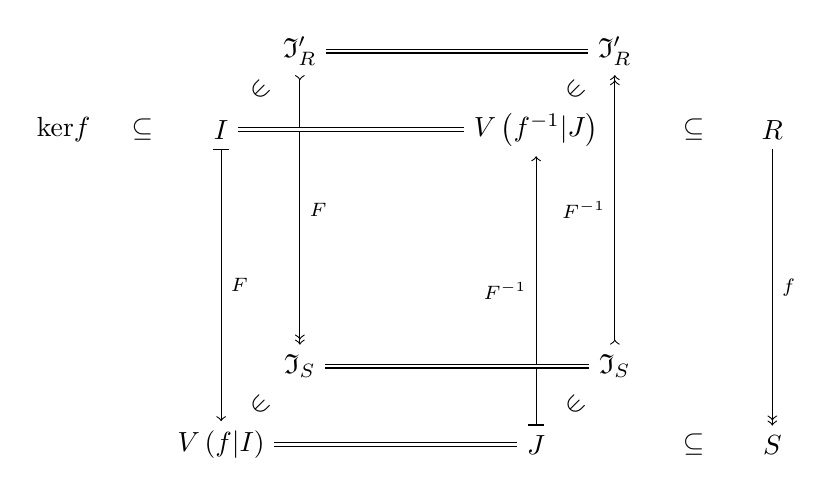
\begin{tikzpicture}[auto]
    \node[rotate=45] (x) at (2.5, 4.5) {$\in $};
    \node[rotate=45] (x) at (2.5, 0.5) {$\in $};
    \node[rotate=45] (x) at (6.5, 0.5) {$\in $};
    \node[rotate=45] (x) at (6.5, 4.5) {$\in $};
    \node (y) at (1, 4) {$\subseteq $};
    \node (y) at (8, 4) {$\subseteq $};
    \node (y) at (8, 0) {$\subseteq $};
    \node (a) at (3, 5) {${\mathfrak I}_R' $};
    \node (b) at (3, 1) {${\mathfrak I}_S $};
    \node (c) at (2, 4) {$I$};
    \node (d) at (2, 0) {$V\left( f|I\right) $};
    \node (e) at (6, 0) {$J$};
    \node (f) at (6, 4) {$V\left( f^{-1} |J\right) $};
    \node (g) at (7, 1) {${\mathfrak I}_S $};
    \node (h) at (7, 5) {${\mathfrak I}_R' $};
    \node (i) at (9, 4) {$R$};
    \node (j) at (9, 0) {$S$};
    \node (k) at (0, 4) {${\rm ker} f$};
    \draw [>->>] (a) to node {$\scriptstyle F$} (b);
    \draw [|->] (c) to node {$\scriptstyle F$} (d);
    \draw [>->>] (g) to node {$\scriptstyle F^{-1} $} (h);
    \draw [|->] (e) to node {$\scriptstyle F^{-1} $} (f);
    \draw [->>] (i) to node {$\scriptstyle f$} (j);
    \draw [double distance=1pt] (c) to node {} (f);
    \draw [double distance=1pt] (d) to node {} (e);
    \draw [double distance=1pt] (a) to node {} (h);
    \draw [double distance=1pt] (b) to node {} (g);
  \end{tikzpicture}
\end{center}
\item
  $\forall I \in \mathfrak{I}_{R}'$に対し、$F(I) = V\left( f|I \right) = J$とおくと、次式のようになり、さらに、${I}/{\ker f} \cong J$が成り立つ。
\begin{center}
  \begin{tikzpicture}[auto]
    \node[rotate=45] (x) at (2.5, 4.5) {$\in $};
    \node[rotate=45] (x) at (2.5, 0.5) {$\in $};
    \node (y) at (1, 4) {$\subseteq $};
    \node (y) at (7, 4) {$\subseteq $};
    \node (y) at (7, 0) {$\subseteq $};
    \node (a) at (3, 5) {${\mathfrak I}_R' $};
    \node (b) at (3, 1) {${\mathfrak I}_S $};
    \node (c) at (2, 4) {$I$};
    \node (d) at (2, 0) {$V\left( f|J\right) $};
    \node (e) at (6, 0) {$J$};
    \node (f) at (12, 4) {$I/{\rm ker} f$};
    \node (i) at (8, 4) {$R$};
    \node (j) at (8, 0) {$S$};
    \node (k) at (0, 4) {${\rm ker} f$};
    \draw [>->>] (a) to node {$\scriptstyle F$} (b);
    \draw [|->] (c) to node {$\scriptstyle F$} (d);
    \draw [>->>] (f) to node {} (e);
    \draw [->>] (i) to node {$\scriptstyle f$} (j);
    \draw [double distance=1pt] (d) to node {} (e);
    \draw [->>] (c)[bend left=10] to node {} (f);
  \end{tikzpicture}
\end{center}
\item
  $\forall I \in \mathfrak{I}_{R}'$に対し、その写像$F:\mathfrak{I}_{R}' \rightarrow \mathfrak{I}_{S};I \mapsto V\left( f|I \right)$が与えられたとき、$F(I) = V\left( f|I \right) = J$とおくと、その左ideal$I$がその環$R$のidealであるならそのときに限り、その左ideal$J$がその環$S$のidealである。
\item
  $\forall I \in \mathfrak{I}_{R}'$に対し、その写像$F:\mathfrak{I}_{R}' \rightarrow \mathfrak{I}_{S};I \mapsto V\left( f|I \right)$が与えられたとき、$F(I) = V\left( f|I \right) = J$とおくと、その左ideal$I$がその環$R$のidealであるなら、次式のようになり、さらに、${R}/{I} \cong {S}/{J}$が成り立つ。
\begin{center}
  \begin{tikzpicture}[auto]
    \node[rotate=45] (x) at (2.5, 4.5) {$\in $};
    \node[rotate=45] (x) at (2.5, 0.5) {$\in $};
    \node (y) at (1, 4) {$\subseteq $};
    \node (y) at (7, 4) {$\subseteq $};
    \node (y) at (7, 0) {$\subseteq $};
    \node (a) at (3, 5) {${\mathfrak I}_R' $};
    \node (b) at (3, 1) {${\mathfrak I}_S $};
    \node (c) at (2, 4) {$I$};
    \node (d) at (2, 0) {$V\left( f|I\right) $};
    \node (e) at (6, 0) {$J$};
    \node (g) at (12, 0) {$S/J$};
    \node (h) at (12, 4) {$R/I$};
    \node (i) at (8, 4) {$R$};
    \node (j) at (8, 0) {$S$};
    \node (k) at (0, 4) {${\rm ker} f$};
    \draw [>->>] (a) to node {$\scriptstyle F$} (b);
    \draw [|->] (c) to node {$\scriptstyle F$} (d);
    \draw [>->>] (h) to node {} (g);
    \draw [->>] (i) to node {$\scriptstyle f$} (j);
    \draw [double distance=1pt] (d) to node {} (e);
    \draw [->>] (i) to node {} (h);
    \draw [->>] (j) to node {} (g);
  \end{tikzpicture} 
\end{center}
\end{itemize}
\end{thm}
\begin{proof}
2つの環々$R$、$S$の間の全射環準同型写像$f:R \twoheadrightarrow S$について、その核$\ker f$を含むその環$R$の左ideal全体の集合を$\mathfrak{I}_{R}'$、その環$S$の左ideal全体の集合を$\mathfrak{I}_{S}$とおきその環$S$の零元を$0_{S}$とおく。次式のように写像$F:\mathfrak{I}_{R}' \rightarrow \mathfrak{I}_{S};I \mapsto V\left( f|I \right) = J$を考えよう。
\begin{center}
  \begin{tikzpicture}[auto]
    \node[rotate=45] (x) at (2.5, 4.5) {$\in $};
    \node[rotate=45] (x) at (2.5, 0.5) {$\in $};
    \node (y) at (1, 4) {$\subseteq $};
    \node (y) at (7, 4) {$\subseteq $};
    \node (y) at (7, 0) {$\subseteq $};
    \node (a) at (3, 5) {${\mathfrak I}_R' $};
    \node (b) at (3, 1) {${\mathfrak I}_S $};
    \node (c) at (2, 4) {$I$};
    \node (d) at (2, 0) {$V\left( f|I\right) $};
    \node (e) at (6, 0) {$J$};
    \node (i) at (8, 4) {$R$};
    \node (j) at (8, 0) {$S$};
    \node (k) at (0, 4) {${\rm ker} f$};
    \draw [->] (a) to node {$\scriptstyle F$} (b);
    \draw [|->] (c) to node {$\scriptstyle F$} (d);
    \draw [->>] (i) to node {$\scriptstyle f$} (j);
    \draw [double distance=1pt] (d) to node {} (e);
  \end{tikzpicture} 
\end{center}
$\forall I \in \mathfrak{I}_{R}'$に対し、定理\ref{3.3.2.22}よりその集合$V\left( f|I \right)$はその環$S$の左idealであるので、$V\left( f|I \right) \in \mathfrak{I}_{S}$が成り立つ。したがって、写像$F:\mathfrak{I}_{R}' \rightarrow \mathfrak{I}_{S};I \mapsto V\left( f|I \right)$が定義できている。ここで、次式のように写像$G:\mathfrak{I}_{S} \rightarrow \mathfrak{I}_{R}';J \mapsto V\left( f^{- 1}|J \right) = I$を考えよう。
\begin{center}
  \begin{tikzpicture}[auto]
    \node[rotate=45] (x) at (2.5, 4.5) {$\in $};
    \node[rotate=45] (x) at (2.5, 0.5) {$\in $};
    \node[rotate=45] (x) at (6.5, 0.5) {$\in $};
    \node[rotate=45] (x) at (6.5, 4.5) {$\in $};
    \node (y) at (1, 4) {$\subseteq $};
    \node (y) at (8, 4) {$\subseteq $};
    \node (y) at (8, 0) {$\subseteq $};
    \node (a) at (3, 5) {${\mathfrak I}_R' $};
    \node (b) at (3, 1) {${\mathfrak I}_S $};
    \node (c) at (2, 4) {$I$};
    \node (d) at (2, 0) {$V\left( f|I\right) $};
    \node (e) at (6, 0) {$J$};
    \node (f) at (6, 4) {$V\left( f^{-1} |J\right) $};
    \node (g) at (7, 1) {${\mathfrak I}_S $};
    \node (h) at (7, 5) {${\mathfrak I}_R' $};
    \node (i) at (9, 4) {$R$};
    \node (j) at (9, 0) {$S$};
    \node (k) at (0, 4) {${\rm ker} f$};
    \draw [->] (a) to node {$\scriptstyle F$} (b);
    \draw [|->] (c) to node {$\scriptstyle F$} (d);
    \draw [->] (g) to node {$\scriptstyle G$} (h);
    \draw [|->] (e) to node {$\scriptstyle G$} (f);
    \draw [->>] (i) to node {$\scriptstyle f$} (j);
    \draw [double distance=1pt] (d) to node {} (e);
    \draw [double distance=1pt] (a) to node {} (h);
    \draw [double distance=1pt] (b) to node {} (g);
  \end{tikzpicture} 
\end{center}
$\forall J \in \mathfrak{I}_{S}$に対し、定理\ref{3.3.2.22}よりその集合$V\left( f^{- 1}|J \right)$はその環$R$の左idealであるかつ、$\forall a \in J$に対し、$- a \in J$が成り立ち、したがって、$a - a = 0_{S} \in J$が成り立つことから、$\ker f = V\left( f^{- 1}|\left\{ 0_{S} \right\} \right) \subseteq V\left( f^{- 1}|J \right)$が成り立つので、$V\left( f^{- 1}|J \right) \in \mathfrak{I}_{R}'$が成り立つ。したがって、写像$G:\mathfrak{I}_{S} \rightarrow \mathfrak{I}_{R}';J \mapsto V\left( f^{- 1}|J \right)$が定義できている。\par
まず、$G \circ F = I_{\mathfrak{I}_{R}'}$が成り立つことを示そう。このとき、$\forall I \in \mathfrak{I}_{R}'$に対し、$V\left( f^{- 1}|V\left( f|I \right) \right) \supseteq I$は明らかに成り立つ。逆に、$\forall a \in R$に対し、$a \in V\left( f^{- 1}|V\left( f|I \right) \right)$が成り立つなら、$V\left( f|V\left( f^{- 1}|V\left( f|I \right) \right) \right) = V\left( f|I \right)$が成り立つので、$f(a) \in V\left( f|I \right)$が成り立ち、$\exists a \in I$に対し、$f(a) = f(b)$が成り立つ。したがって、次のようになり、
\begin{align*}
f(a) = f(b) &\Leftrightarrow f(a) - f(b) = f(a) + f( - b) = f(a - b) = 0_{S}\\
&\Leftrightarrow a - b \in \ker f
\end{align*}
したがって、次のようになる。
\begin{align*}
(a - b) + b &= a + 0\\
&= a \in I
\end{align*}
以上より、$V\left( f^{- 1}|V\left( f|I \right) \right) \subseteq I$が成り立つ。したがって、$G \circ F(I) = V\left( f^{- 1}|V\left( f|I \right) \right) = I$が成り立つので、$G \circ F = I_{\mathfrak{I}_{R}'}$が得られた。\par
次に、$F \circ G = I_{\mathfrak{I}_{S}}$が成り立つことを示そう。もちろん、$\forall J \in \mathfrak{I}_{S}$に対し、$V\left( f|V\left( f^{- 1}|J \right) \right) \subseteq J$は成り立つ。逆に、$\forall a \in S$に対し、$a \in J$が成り立つなら、その写像$f$は全射であるので、$\exists b \in R$に対し、$f(b) = a$が成り立つ。$a \in J$より$V\left( f^{- 1}|\left\{ a \right\} \right) \subseteq V\left( f^{- 1}|J \right)$が成り立つので、$b \in V\left( f^{- 1}|\left\{ a \right\} \right) \subseteq V\left( f^{- 1}|J \right)$が成り立ち、したがって、$f(b) = a \in V\left( f|V\left( f^{- 1}|J \right) \right)$が成り立つ。以上より、$J \subseteq V\left( f|V\left( f^{- 1}|J \right) \right)$が成り立つ。したがって、$F \circ G(J) = V\left( f|V\left( f^{- 1}|J \right) \right) = J$が成り立つので、$F \circ G = I_{\mathfrak{I}_{S}}$が得られた。\par
以上より、$G \circ F = I_{\mathfrak{I}_{R}'}$かつ$F \circ G = I_{\mathfrak{I}_{S}}$が成り立つ。このようなその写像$G:\mathfrak{I}_{S} \rightarrow \mathfrak{I}_{R}'$が存在するので、その写像$F:\mathfrak{I}_{R}' \rightarrow \mathfrak{I}_{S}$は全単射でその写像$G$はその写像$F$の逆写像である。よって、その写像$F:\mathfrak{I}_{R}' \rightarrow \mathfrak{I}_{S};I \mapsto V\left( f|I \right) = J$は全単射でその逆写像$F^{- 1}$が$F^{- 1}:\mathfrak{I}_{S} \rightarrow \mathfrak{I}_{R}';J \mapsto V\left( f^{- 1}|J \right) = I$と与えられる。\par
また、$\forall I \in \mathfrak{I}_{R}'$に対し、写像$f':I \rightarrow V\left( f|I \right);a \mapsto f(a)$を考え$F(I) = V\left( f|I \right) = J$とおくと、この写像$f'$は明らかに全射環準同型写像であるから、次式のように考えられると、
\begin{center}
  \begin{tikzpicture}[auto]
    \node[rotate=45] (x) at (2.5, 4.5) {$\in $};
    \node[rotate=45] (x) at (2.5, 0.5) {$\in $};
    \node[rotate=45] (x) at (6.5, 4.5) {$\in $};
    \node (a) at (3, 5) {$I$};
    \node (b) at (3, 1) {$I/{\rm ker} f' $};
    \node (c) at (2, 4) {$a$};
    \node (d) at (2, 0) {$a+{\rm ker} f' $};
    \node (f) at (6, 4) {$f\left( a\right) $};
    \node (g) at (7, 1) {$V\left( f'|I\right) $};
    \node (h) at (7, 5) {$J$};
    \draw [->>] (a) to node {} (b);
    \draw [|->] (c) to node {} (d);
    \draw [->>] (a) to node {$\scriptstyle f'$} (h);
    \draw [|->] (c) to node {$\scriptstyle f'$} (f);
    \draw [double distance=1pt] (g) to node {} (h);
  \end{tikzpicture} 
\end{center}
環準同型定理より次式が成り立つので、
\begin{center}
  \begin{tikzpicture}[auto]
    \node[rotate=45] (x) at (2.5, 4.5) {$\in $};
    \node[rotate=45] (x) at (2.5, 0.5) {$\in $};
    \node[rotate=45] (x) at (6.5, 4.5) {$\in $};
    \node (a) at (3, 5) {$I$};
    \node (b) at (3, 1) {$I/{\rm ker} f' $};
    \node (c) at (2, 4) {$a$};
    \node (d) at (2, 0) {$a+{\rm ker} f' $};
    \node (f) at (6, 4) {$f\left( a\right) $};
    \node (g) at (7, 1) {$V\left( f'|I\right) $};
    \node (h) at (7, 5) {$J$};
    \draw [->>] (a) to node {} (b);
    \draw [|->] (c) to node {} (d);
    \draw [->>] (a) to node {$\scriptstyle f'$} (h);
    \draw [|->] (c) to node {$\scriptstyle f'$} (f);
    \draw [double distance=1pt] (g) to node {} (h);
    \draw [>->>] (b) to node {} (g);
  \end{tikzpicture} 
\end{center}
次式のようになり、
\begin{center}
  \begin{tikzpicture}[auto]
    \node[rotate=45] (x) at (2.5, 4.5) {$\in $};
    \node[rotate=45] (x) at (2.5, 0.5) {$\in $};
    \node (y) at (1, 4) {$\subseteq $};
    \node (y) at (7, 4) {$\subseteq $};
    \node (y) at (7, 0) {$\subseteq $};
    \node (a) at (3, 5) {${\mathfrak I}_R' $};
    \node (b) at (3, 1) {${\mathfrak I}_S $};
    \node (c) at (2, 4) {$I$};
    \node (d) at (2, 0) {$V\left( f|I\right) $};
    \node (e) at (6, 0) {$J$};
    \node (f) at (12, 4) {$I/{\rm ker} f'$};
    \node (i) at (8, 4) {$R$};
    \node (j) at (8, 0) {$S$};
    \node (k) at (0, 4) {${\rm ker} f$};
    \node (l) at (12, 0) {$V\left( f'|I\right) $};
    \draw [>->>] (a) to node {$\scriptstyle F$} (b);
    \draw [|->] (c) to node {$\scriptstyle F$} (d);
    \draw [>->>] (f) to node {} (l);
    \draw [->>] (i) to node {$\scriptstyle f$} (j);
    \draw [double distance=1pt] (d) to node {} (e);
    \draw [->>] (c)[bend left=10] to node {} (f);
  \end{tikzpicture} 
\end{center}
${I}/{\ker f'} \cong V\left( f'|I \right)$が得られる。ここで、$V\left( f'|I \right) = V\left( f|I \right) = J$が成り立つかつ、$\ker f' = \ker f$が成り立つので、次式のようになり、
\begin{center}
  \begin{tikzpicture}[auto]
    \node[rotate=45] (x) at (2.5, 4.5) {$\in $};
    \node[rotate=45] (x) at (2.5, 0.5) {$\in $};
    \node (y) at (1, 4) {$\subseteq $};
    \node (y) at (7, 4) {$\subseteq $};
    \node (y) at (7, 0) {$\subseteq $};
    \node (a) at (3, 5) {${\mathfrak I}_R' $};
    \node (b) at (3, 1) {${\mathfrak I}_S $};
    \node (c) at (2, 4) {$I$};
    \node (d) at (2, 0) {$V\left( f|J\right) $};
    \node (e) at (6, 0) {$J$};
    \node (f) at (12, 4) {$I/{\rm ker} f$};
    \node (i) at (8, 4) {$R$};
    \node (j) at (8, 0) {$S$};
    \node (k) at (0, 4) {${\rm ker} f$};
    \draw [>->>] (a) to node {$\scriptstyle F$} (b);
    \draw [|->] (c) to node {$\scriptstyle F$} (d);
    \draw [>->>] (f) to node {} (e);
    \draw [->>] (i) to node {$\scriptstyle f$} (j);
    \draw [double distance=1pt] (d) to node {} (e);
    \draw [->>] (c)[bend left=10] to node {} (f);
  \end{tikzpicture}
\end{center}
${I}/{\ker f} \cong J$が成り立つ。\par
$\forall I \in \mathfrak{I}_{R}'$に対し、その写像$F:\mathfrak{I}_{R}' \rightarrow \mathfrak{I}_{S};I \mapsto V\left( f|I \right)$が与えられたとき、$F(I) = V\left( f|I \right) = J$とおくと、定理\ref{3.3.2.22}よりその左ideal$I$がその環$R$のidealであるならそのときに限り、その左ideal$J$がその環$S$のidealであることが直ちに分かる。\par
$\forall I \in \mathfrak{I}_{R}'$に対し、その写像$F:\mathfrak{I}_{R}' \rightarrow \mathfrak{I}_{S};I \mapsto V\left( f|I \right)$が与えられたとき、$F(I) = V\left( f|I \right) = J$とおくと、その左ideal$I$がその環$R$のidealであるなら、上記の議論により集合$J$はその環$S$のidealで次式のように自然な全射環準同型写像$\varphi_{S}:S \twoheadrightarrow {S}/{J}$を考えると、
\begin{center}
  \begin{tikzpicture}[auto]
    \node[rotate=45] (x) at (2.5, 4.5) {$\in $};
    \node[rotate=45] (x) at (2.5, 0.5) {$\in $};
    \node (y) at (1, 4) {$\subseteq $};
    \node (y) at (7, 4) {$\subseteq $};
    \node (y) at (7, 0) {$\subseteq $};
    \node (a) at (3, 5) {${\mathfrak I}_R' $};
    \node (b) at (3, 1) {${\mathfrak I}_S $};
    \node (c) at (2, 4) {$I$};
    \node (d) at (2, 0) {$V\left( f|I\right) $};
    \node (e) at (6, 0) {$J$};
    \node (g) at (12, 0) {$S/J$};
    \node (i) at (8, 4) {$R$};
    \node (j) at (8, 0) {$S$};
    \node (k) at (0, 4) {${\rm ker} f$};
    \draw [>->>] (a) to node {$\scriptstyle F$} (b);
    \draw [|->] (c) to node {$\scriptstyle F$} (d);
    \draw [->>] (i) to node {$\scriptstyle f$} (j);
    \draw [double distance=1pt] (d) to node {} (e);
    \draw [->>] (j) to node {$\scriptstyle \varphi_S $} (g);
  \end{tikzpicture} 
\end{center}
$J = \ker\varphi_{S}$が成り立ち、$\varphi_{S} \circ f = \rho$とおくと、その写像$\rho$は次式のように全射環準同型写像で、
\begin{center}
  \begin{tikzpicture}[auto]
    \node[rotate=45] (x) at (2.5, 4.5) {$\in $};
    \node[rotate=45] (x) at (2.5, 0.5) {$\in $};
    \node (y) at (1, 4) {$\subseteq $};
    \node (y) at (7, 4) {$\subseteq $};
    \node (y) at (7, 0) {$\subseteq $};
    \node (a) at (3, 5) {${\mathfrak I}_R' $};
    \node (b) at (3, 1) {${\mathfrak I}_S $};
    \node (c) at (2, 4) {$I$};
    \node (d) at (2, 0) {$V\left( f|I\right) $};
    \node (e) at (6, 0) {$J$};
    \node (g) at (12, 0) {$S/J$};
    \node (i) at (8, 4) {$R$};
    \node (j) at (8, 0) {$S$};
    \node (k) at (0, 4) {${\rm ker} f$};
    \draw [>->>] (a) to node {$\scriptstyle F$} (b);
    \draw [|->] (c) to node {$\scriptstyle F$} (d);
    \draw [->>] (i) to node {$\scriptstyle f$} (j);
    \draw [double distance=1pt] (d) to node {} (e);
    \draw [->>] (j) to node {$\scriptstyle \varphi_S $} (g);
    \draw [->>] (i) to node {$\scriptstyle \rho $} (g);
  \end{tikzpicture} 
\end{center}
$\forall a \in R$に対し、$a \in \ker\rho$が成り立つならそのときに限り、$\rho(a) = f(a) + J = J$が成り立ち、これが成り立つならそのときに限り、$f(a) \in J$が成り立つ、即ち、$a \in V\left( f^{- 1}|J \right)$が成り立つ。ここで、上記の議論により$a \in F^{- 1}(J) = I$が成り立つので、$\ker\rho = I$が得られる。以上より、自然な全射環準同型写像$\varphi_{R}:R \twoheadrightarrow {R}/{\ker\rho}$を用いれば、次式のように与えられ、
\begin{center}
  \begin{tikzpicture}[auto]
    \node[rotate=45] (x) at (2.5, 4.5) {$\in $};
    \node[rotate=45] (x) at (2.5, 0.5) {$\in $};
    \node[rotate=45] (x) at (6.5, 4.5) {$\in $};
    \node (a) at (3, 5) {$R$};
    \node (b) at (3, 1) {$R/{\rm ker} \rho $};
    \node (c) at (2, 4) {$a$};
    \node (d) at (2, 0) {$a+{\rm ker} \rho $};
    \node (f) at (6, 4) {$f\left( a\right) +J$};
    \node (g) at (7, 1) {$V\left( \rho \right) $};
    \node (h) at (7, 5) {$S/J$};
    \draw [->>] (a) to node {$\scriptstyle \varphi_R $} (b);
    \draw [|->] (c) to node {$\scriptstyle \varphi_R $} (d);
    \draw [->>] (a) to node {$\scriptstyle \rho $} (h);
    \draw [|->] (c) to node {$\scriptstyle \rho $} (f);
    \draw [double distance=1pt] (g) to node {} (h);
  \end{tikzpicture} 
\end{center}
$\ker\rho = I$かつ${S}/{J} = V(\rho)$が成り立つことに注意すれば、環準同型定理より次のようになるので、
\begin{center}
  \begin{tikzpicture}[auto]
    \node[rotate=45] (x) at (2.5, 4.5) {$\in $};
    \node[rotate=45] (x) at (2.5, 0.5) {$\in $};
    \node[rotate=45] (x) at (6.5, 4.5) {$\in $};
    \node (a) at (3, 5) {$R$};
    \node (b) at (3, 1) {$R/I$};
    \node (c) at (2, 4) {$a$};
    \node (d) at (2, 0) {$a+I$};
    \node (f) at (6, 4) {$f\left( a\right) +J$};
    \node (g) at (7, 1) {$S/J$};
    \node (h) at (7, 5) {$S/J$};
    \draw [->>] (a) to node {$\scriptstyle \varphi_R $} (b);
    \draw [|->] (c) to node {$\scriptstyle \varphi_R $} (d);
    \draw [->>] (a) to node {$\scriptstyle \rho $} (h);
    \draw [|->] (c) to node {$\scriptstyle \rho $} (f);
    \draw [double distance=1pt] (g) to node {} (h);
    \draw [>->>] (b) to node {} (g);
  \end{tikzpicture} 
\end{center}
次式が成り立ち
\begin{center}
  \begin{tikzpicture}[auto]
    \node[rotate=45] (x) at (2.5, 4.5) {$\in $};
    \node[rotate=45] (x) at (2.5, 0.5) {$\in $};
    \node (y) at (1, 4) {$\subseteq $};
    \node (y) at (7, 4) {$\subseteq $};
    \node (y) at (7, 0) {$\subseteq $};
    \node (a) at (3, 5) {${\mathfrak I}_R' $};
    \node (b) at (3, 1) {${\mathfrak I}_S $};
    \node (c) at (2, 4) {$I$};
    \node (d) at (2, 0) {$V\left( f|I\right) $};
    \node (e) at (6, 0) {$J$};
    \node (g) at (12, 0) {$S/J$};
    \node (h) at (12, 4) {$R/I$};
    \node (i) at (8, 4) {$R$};
    \node (j) at (8, 0) {$S$};
    \node (k) at (0, 4) {${\rm ker} f$};
    \draw [>->>] (a) to node {$\scriptstyle F$} (b);
    \draw [|->] (c) to node {$\scriptstyle F$} (d);
    \draw [>->>] (h) to node {} (g);
    \draw [->>] (i) to node {$\scriptstyle f$} (j);
    \draw [double distance=1pt] (d) to node {} (e);
    \draw [->>] (i) to node {} (h);
    \draw [->>] (j) to node {} (g);
  \end{tikzpicture} 
\end{center}
${R}/{I} \cong {S}/{J}$が成り立つ。
\end{proof}
%\hypertarget{ux6975ux5927ideal}{%
\subsubsection{極大ideal}%\label{ux6975ux5927ideal}}
\begin{dfn}
環$R$のこれ自身でない左ideal$J$を含むその環$R$の左idealがその環$R$とその左ideal$J$以外に存在しないとき、その左ideal$J$をその環$R$の極大左idealという。同様に、環$R$のこれ自身でない右ideal$J$を含むその環$R$の右idealがその環$R$とその右ideal$J$以外に存在しないとき、その右ideal$J$をその環$R$の極大右idealという。
\end{dfn}
\begin{thm}\label{3.3.2.24}
可換環$R$が与えられたとき、その環$R$の極大左idealと極大右idealとは一致する。
\end{thm}
\begin{dfn}
可換環$R$での極大左idealを単に極大idealという。
\end{dfn}
\begin{proof}
可換環$R$が与えられたとき、その環$R$の極大左ideal$J$について、$\forall a \in J\forall r \in R$に対し、$ra = ar \in J$が成り立つので、その極大左ideal$J$はその環$R$の右idealでもある。ここで、これを含むその環$R$自身、その右ideal$J$自身でないその環$R$の右ideal$J'$が存在したとすれば、その環は乗法について可換的なので、$\forall a \in J'\forall r \in R$に対し、$ar = ra \in J'$が成り立つので、その右ideal$J'$はその環$R$の左idealでもあり$J \subset J'$が成り立つが、これはその左ideal$J$がその環$R$の極大左idealであることに矛盾する。したがって、その極大左ideal$J$はその環$R$の極大右idealでもある。極大右idealについても同様にして示される。
\end{proof}
\begin{thm}\label{3.3.2.25}
環$R$のこれ自身でないideal$J$が与えられたとき、次のことは同値である。
\begin{itemize}
\item
  その商環${R}/{J}$は斜体である。
\item
  そのideal$J$はその環$R$の極大左idealである。
\item
  そのideal$J$はその環$R$の極大右idealである。
\end{itemize}
\end{thm}
\begin{proof}
環$R$のこれ自身でないideal$J$が与えられたとき、その商環${R}/{J}$が斜体であるならそのときに限り、定理\ref{3.3.2.4}よりその商環${R}/{J}$はこれ自身か零ideal以外の左idealをもたないので、これが成り立つならそのときに限り、自然な全射環準同型写像$\varphi:R \rightarrow {R}/{J}$は全射であるから、定理\ref{3.3.2.23}より次のようになる。
\begin{align*}
V\left( \varphi^{- 1}|{R}/{J} \right) = R,\ \ V\left( \varphi^{- 1}|\left( {R}/{J} \right)0 \right) = J
\end{align*}
これがその左ideal$J$を含むその環$R$の左ideal全てであるから、そのideal$J$はその環$R$の極大左idealである。ゆえに、次のことは同値である。
\begin{itemize}
\item
  その商環${R}/{J}$は斜体である。
\item
  そのideal$J$はその環$R$の極大左idealである。
\end{itemize}
同様にして次のことは同値であることが示される。
\begin{itemize}
\item
  その商環${R}/{J}$は斜体である。
\item
  そのideal$J$はその環$R$の極大左idealである。
\end{itemize}
\end{proof}
\begin{thm}\label{3.3.2.26}
可換環$R$のこれ自身でないideal$J$が与えられたとき、その商環${R}/{J}$が斜体であるならそのときに限り、そのideal$J$はその環$R$の極大idealである。
\end{thm}
\begin{proof}
可換環$R$のこれ自身でないideal$J$が与えられたとき、その商環${R}/{J}$が斜体であるならそのときに限り、定理\ref{3.3.2.25}よりそのideal$J$はその環$R$の極大左idealであった。ここで、定理\ref{3.3.2.24}よりその極大左ideal$J$はその環$R$の極大idealでもある。
\end{proof}
%\hypertarget{ux7d20ideal}{%
\subsubsection{素ideal}%\label{ux7d20ideal}}
\begin{dfn}
可換環$R$のideal$P$がその環$R$自身でなく、$\forall a,b \in R$に対し、$ab \in P$が成り立つなら、$a \in P$または$b \in P$が成り立つとき、そのideal$P$をその環$R$の素idealという。
\end{dfn}
\begin{thm}\label{3.3.2.27}
可換環$R$のideal$P$が与えられたとき、そのideal$P$がその環$R$の素idealであるならそのときに限り、その商環${R}/{P}$は整域である。
\end{thm}
\begin{proof}
可換環$R$のideal$P$が与えられたとき、その商環${R}/{P}$はもちろん可換環である。そのideal$P$がその環$R$の素idealであるなら、$\exists a + P,b + P \in {R}/{P}$に対し、$a + P \neq P$かつ$b + P \neq P$が成り立つかつ、$(a + P)(b + P) = P$が成り立つと仮定しよう。このとき、次のようになるので、
\begin{align*}
(a + P)(b + P) = ab + P = P
\end{align*}
$ab \equiv 0\ \mathrm{mod}P $が成り立つ、即ち、$ab \in P$が成り立つので、$a \in P$または$b \in P$が成り立つ。ここで、$a \in P$とすれば、$a \equiv 0\ \mathrm{mod}P $が成り立つ、即ち、$a + P = P$が成り立つことになるが、これは仮定に矛盾する。$b \in P$についても同様であるから、$a + P \neq P$かつ$b + P \neq P$が成り立つかつ、$(a + P)(b + P) = P$が成り立つことは矛盾している。したがって、$\forall a + P,b + P \in {R}/{P}$に対し、$a + P \neq P$かつ$b + P \neq P$が成り立つなら、$(a + P)(b + P) \neq P$が成り立つことになる、即ち、その商環${R}/{P}$は整域である。\par
逆に、その商環${R}/{P}$が整域であるとすると、$\forall a,b \in P$に対し、$a \notin P$かつ$b \notin P$が成り立つなら、$a \equiv 0\ \mathrm{mod}P $または$b \equiv 0\ \mathrm{mod}P $が成り立たないので、$a + P \neq P$かつ$b + P \neq P$が成り立ち、したがって、$(a + P)(b + P) \neq P$が成り立つことになる。ゆえに、$ab + P \neq P$が成り立つので、$ab \equiv 0\ \mathrm{mod}P $が成り立たない、即ち、$ab \notin P$が成り立つことになる。対偶律よりそのideal$P$は素idealでもある。
\end{proof}
\begin{thm}\label{3.3.2.28}
可換環$R$の極大idealは素idealである。
\end{thm}
\begin{proof} 可換環$R$の極大ideal$P$が与えられたとき、定理\ref{3.3.2.26}よりその商環${R}/{P}$は斜体であり、さらに、零因子をもたない。また、その環$R$は乗法について可換的で、もちろん、その商環${R}/{P}$も可換的であるので、その商環${R}/{P}$は整域である。定理\ref{3.3.2.27}よりよって、可換環$R$の極大ideal$P$は素idealである。
\end{proof}
%\hypertarget{ux5546ux306eux4f53}{%
\subsubsection{商の体}%\label{ux5546ux306eux4f53}}
\begin{thm}\label{3.3.2.29}
体$K$の部分環$K'$が与えられたとき、その環$K'$は整域である。
\end{thm}
\begin{proof}
体$K$の部分環$K'$が与えられたとき、$\forall a,b \in K'$に対し、$a,b \in K$が成り立つので、$ab = ba$が成り立つ。したがって、その環$K'$は可換環である。さらに、その環$K'$が零因子をもつとすれば、その零因子はその体$K$の元でもあるので、体の定義に矛盾する。したがって、その環$K'$は零因子をもたない。ゆえに、その環$K'$は整域である。
\end{proof}
\begin{thm}\label{3.3.2.30}
零環でない環$R$から体$K$への単射環準同型写像$f:R \rightarrow K$が存在するなら、その環$R$は整域である。
\end{thm}
\begin{proof}
零環でない環$R$から体$K$への単射環準同型写像$f:R \rightarrow K$が存在するなら、その値域$V(f)$は定理\ref{3.3.2.17}よりその体$K$の部分環であり、定理\ref{3.3.2.29}よりその環$V(f)$は整域である。ここで、写像$f':R \rightarrow V(f);a \mapsto f(a)$は全単射で、さらに、環同型写像でもある。したがって、環同型写像${f'}^{- 1}:V(f) \rightarrow R$が存在し$\forall a,b \in R$に対し、次のようになる。
\begin{align*}
ab &= f^{- 1} \circ f(ab)\\
&= f^{- 1}\left( f(ab) \right)\\
&= f^{- 1}\left( f(a)f(b) \right)\\
&= f^{- 1}\left( f(b)f(a) \right)\\
&= f^{- 1}\left( f(ba) \right)\\
&= f^{- 1} \circ f(ba) = ba
\end{align*}
ゆえに、その環$R$は可換環である。\par
さらに、その環$R$が零因子をもつと仮定すると、$\exists a,b \in R$に対し、$a \neq 0$かつ$b \neq 0$が成り立つなら、$ab = 0$が成り立つことになる。このとき、$f(a) \neq 0$かつ$f(b) \neq 0$が成り立ち、したがって、$f(a)f(b) = f(ab) = f(0) = 0$が成り立つによりその環$V(f)$は零因子をもつことになるが、これはその環$V(f)$が整域であることに矛盾する。ゆえに、その環$R$は零因子をもたない。\par
以上よりよって、その環$R$は整域である。
\end{proof}
\begin{dfn}
2つの環々$R_{1}$、$R_{2}$の間の単射環準同型写像$f:R_{1} \rightarrow R_{2}$が与えられたとき、その値域$V(f)$はその環$R_{2}$の部分環となるのであった。ここで、その値域$V(f)$をその環$R_{1}$と同一視するとき、その写像$f$をその環$R_{1}$のその環$R_{2}$への埋め込みという。このような埋め込みが存在するとき、その環$R_{1}$はその環$R_{2}$へ埋め込み可能であるという。
\end{dfn}
\begin{dfn}
体$K$の部分環$K'$が与えられたとき、$\forall a,b \in K'$に対し、$a\frac{1}{b}$を$\frac{a}{b}$と書く。
\end{dfn}
\begin{thm}\label{3.3.2.31}
体$K$の部分環$K'$が与えられたとき、$\forall a,b,c,d \in K'$に対し、定義可能であるかぎり次式が成り立つ。
\begin{align*}
\frac{a}{b} + \frac{c}{d} = \frac{ad + bc}{bd},\ \ \frac{a}{b}\frac{c}{d} = \frac{ac}{bd}
\end{align*}
\end{thm}
\begin{proof}
体$K$の部分環$K'$が与えられたとき、$\forall a,b,c,d \in K'$に対し、定義可能であるかぎり次のようになる。
\begin{align*}
\frac{a}{b} + \frac{c}{d} &= a\frac{1}{b} + c\frac{1}{d}\\
&= ad\frac{1}{d}\frac{1}{b} + cb\frac{1}{b}\frac{1}{d}\\
&= ad\frac{1}{bd} + cb\frac{1}{db}\\
&= ad\frac{1}{bd} + bc\frac{1}{bd}\\
&= (ad + bc)\frac{1}{bd}\\
&= \frac{ad + bc}{bd}\\
\frac{a}{b}\frac{c}{d} &= a\frac{1}{b}c\frac{1}{d}\\
&= ac\frac{1}{b}\frac{1}{d}\\
&= ac\frac{1}{db}ac\frac{1}{bd}\\
&= \frac{ac}{bd}
\end{align*}
\end{proof}
\begin{thm}\label{3.3.2.32}
体$K$の部分環$K'$が与えられたとき、次式のようにして定義される集合$L$は
\begin{align*}
L = \left\{ \frac{a}{b} \in K \middle| a,b \in K' \right\}
\end{align*}
その体$K$の部分体である。さらに、その集合$L$はその部分環$K'$を含むその体$K$の部分体たちのうち順序関係$\subseteq$の意味で最小なものである。
\end{thm}
\begin{dfn}
その集合$L$をその部分環$K'$のその体$K$における商の体、分数体という。
\end{dfn}
\begin{proof}
体$K$の部分環$K'$が与えられたとき、次式のようにして定義される集合$L$について、
\begin{align*}
L = \left\{ \frac{a}{b} \in K \middle| a,b \in K',\ \ b \neq 0 \right\}
\end{align*}
定理\ref{3.3.1.14}より$1 \in K'$が成り立つので、$\frac{1}{1} = 1 \in L$が成り立つ。さらに、$\forall\frac{a}{b},\frac{c}{d} \in L$に対し、$- a \in K'$が成り立つので、$- \frac{a}{b} = \frac{- a}{b} \in L$が成り立つかつ、定理\ref{3.3.2.31}より$\frac{a}{b} + \frac{c}{d},\frac{a}{b}\frac{c}{d} \in L$が成り立つので、定理\ref{3.3.1.14}よりその集合$L$はその体$K$の部分環である。さらに、$\forall\frac{a}{b},\frac{c}{d} \in L$に対し、次のようになることから、
\begin{align*}
\frac{a}{b}\frac{c}{d} = \frac{ac}{bd} = \frac{ca}{db} = \frac{c}{d}\frac{a}{b}
\end{align*}
その部分環$L$は可換環である。ここで、$\forall\frac{a}{b} \in L$に対し、$\frac{a}{b} \neq 0$が成り立つなら、$a \neq 0$かつ$\frac{1}{b} \neq 0$が成り立つ。$a \in K$が成り立つので、元$\frac{1}{a}$がその体$K$に存在し$\frac{b}{a} \in L$が成り立つ。ゆえに、その部分環$L$は斜体である。よって、その集合$L$はその体$K$の部分体である。\par
さらに、$\forall a \in K'$に対し、$a = \frac{a}{1} \in L$が成り立つので、$K' \subseteq L$が成り立つ。ここで、その集合$L$はその部分環$K'$を含むその体$K$の部分体$K''$が与えられたとき、$\forall\frac{a}{b} \in L$に対し、$a,b \in K'$が成り立つので、$a,b \in K''$が成り立ち、$b \neq 0$より体の定義より$\frac{1}{b} \in K''$が成り立つことになる。定理\ref{3.3.1.14}より$\frac{a}{b} = a\frac{1}{b} \in K''$が成り立つことになるので、$L \subseteq K''$が成り立つ。よって、その集合$L$はその部分環$K'$を含むその体$K$の部分体たちのうち順序関係$\subseteq$の意味で最小なものである。
\end{proof}
%\hypertarget{ux6574ux57dfux304bux3089ux306eux57cbux3081ux8fbcux307fux306bux3088ux308bux4f53ux306eux69cbux6210}{%
\subsubsection{整域からの埋め込みによる体の構成}%\label{ux6574ux57dfux304bux3089ux306eux57cbux3081ux8fbcux307fux306bux3088ux308bux4f53ux306eux69cbux6210}}
\begin{thm}\label{3.3.2.33}
整域$R$が与えられたとき、次のことを満たすような体$L$と環準同型写像$\varphi:R \rightarrow L$が存在する。
\begin{itemize}
\item
  その写像$\varphi$はその整域$R$のその体$L$への埋め込みである。
\item
  $\forall l \in L$に対し、その整域$R$の元々$a$、$b$が存在して$b \neq 0$が成り立つかつ、$l = \frac{\varphi(a)}{\varphi(b)}$が成り立つ。
\end{itemize}\par
詳しくいえば、その体$L$は、集合$R \times R \setminus \left\{ 0 \right\}$の元々$\left( a,b \right)$、$\left( c,d \right)$に対し、$ad = cb$が成り立つとき、$\left( a,b \right)D\left( c,d \right)$と関係$D$が定義されたときの商集合${\left( R \times R \setminus \left\{ 0 \right\} \right)}/{D}$で、$\forall C_{D}(a,b),C_{D}(c,d) \in {\left( R \times R \setminus \left\{ 0 \right\} \right)}/{D}$に対し、次式のように定義される。
\begin{align*}
C_{D}(a,b) + C_{D}(c,d) = C_{D}(ad + bc,bd),\ \ C_{D}(a,b)C_{D}(c,d) = C_{D}(ac,bd)
\end{align*}
このときの零元、単位元はそれぞれ$C_{D}(0,1)$、$C_{D}(1,1)$である。また、その写像$\varphi$も次式のように定義される。
\begin{align*}
\varphi:R \rightarrow L;a \mapsto C_{D}(a,1)
\end{align*}
\end{thm}
\begin{dfn}
このときの体$L$をその整域$R$の商の体、分数体という。
\end{dfn}
\begin{proof}
整域$R$が与えられたとき、集合$R \times R \setminus \left\{ 0 \right\}$の元々$(a,b)$、$(c,d)$に対し、$ad = cb$が成り立つとき、$(a,b)D(c,d)$と関係$D$が定義される。このとき、$ab = ab$が成り立つので、$(a,b)D(a,b)$が成り立つ。$(a,b)D(c,d)$が成り立つなら、$ad = cb$が成り立つならそのときに限り、$cb = ad$が成り立つので、$(c,d)D(a,b)$が成り立つ。最後に、$(a,b)D(c,d)$かつ$(c,d)D(e,f)$が成り立つなら、$ad = cb$かつ$cf = ed$が成り立つので、$adf = cbf = cfb = edb$が成り立ち、したがって、$adf - edb = (af - eb)d = 0$が成り立つ。ここで、その環$R$は整域であるから、$d \neq 0$より$af - eb = 0$が成り立つ。ゆえに、$af = eb$が得られ$(a,b)D(e,f)$が成り立つので、その関係$D$は同値関係である。\par
したがって、商集合${\left( R \times R \setminus \left\{ 0 \right\} \right)}/{D}$が得られる。ここで、$\forall C_{D}(a,b),C_{D}(c,d) \in {\left( R \times R \setminus \left\{ 0 \right\} \right)}/{D}$に対し、次式のように定義されるとする。
\begin{align*}
C_{D}(a,b) + C_{D}(c,d) = C_{D}(ad + bc,bd),\ \ C_{D}(a,b)C_{D}(c,d) = C_{D}(ac,bd)
\end{align*}
このとき、$C_{D}(a,b) = C_{D}\left( a',b' \right)$かつ$C_{D}(c,d) = C_{D}\left( c',d' \right)$が成り立つなら、次のようになることから、
\begin{align*}
(ad + bc)b'd' &= ab'dd' + bb'cd'\\
&= a'bdd' + bb'c'd\\
&= \left( a'd' + b'c' \right)bd\\
acb'd' &= ab'cd'\\
&= a'bc'd\\
&= a'c'bd
\end{align*}
次式が成り立つ。
\begin{align*}
C_{D}(a,b) + C_{D}(c,d) &= C_{D}(ad + bc,bd)\\
&= C_{D}\left( a'd' + b'c',b'd' \right)\\
&= C_{D}\left( a',b' \right) + C_{D}\left( c',d' \right)\\
C_{D}(a,b)C_{D}(c,d) &= C_{D}(ac,bd)\\
&= C_{D}\left( a'c',b'd' \right)\\
&= C_{D}\left( a',b' \right)C_{D}\left( c',d' \right)
\end{align*}\par
ここで、$\forall C_{D}(a,b),C_{D}(c,d),C_{D}(e,f) \in {\left( R \times R \setminus \left\{ 0 \right\} \right)}/{D}$に対し、次のようになるので、
\begin{align*}
\left( C_{D}(a,b) + C_{D}(c,d) \right) + C_{D}(e,f) &= C_{D}(ad + bc,bd) + C_{D}(e,f)\\
&= C_{D}\left( (ad + bc)f + bde,bdf \right)\\
&= C_{D}(adf + cfb + ebd,bdf)\\
&= C_{D}\left( dfa + (cf + de)b,bdf \right)\\
&= C_{D}(a,b) + C_{D}(cf + de,df)\\
&= C_{D}(a,b) + \left( C_{D}(c,d) + C_{D}(e,f) \right)\\
C_{D}(a,b) + C_{D}(0,1) &= C_{D}(a1 + b0,b1) = C_{D}(a,b)\\
C_{D}(0,1) + C_{D}(a,b) &= C_{D}(0b + 1a,1b) = C_{D}(a,b)\\
C_{D}(a,b) + C_{D}( - a,b) &= C_{D}\left( ab - ba,b^{2} \right) = C_{D}(0,1)\\
C_{D}( - a,b) + C_{D}(a,b) &= C_{D}\left( - ab + ba,b^{2} \right) = C_{D}(0,1)\\
C_{D}(a,b) + C_{D}(c,d) &= C_{D}(ad + bc,bd)\\
&= C_{D}(cb + da,db)\\
&= C_{D}(c,d) + C_{D}(a,b)
\end{align*}
その組$\left( {\left( R \times R \setminus \left\{ 0 \right\} \right)}/{D}, + \right)$は可換群をなす。さらに、次のようになるので、
\begin{align*}
\left( C_{D}(a,b)C_{D}(c,d) \right)C_{D}(e,f) &= C_{D}(ac,bd)C_{D}(e,f)\\
&= C_{D}\left( (ac)e,(bd)f \right)\\
&= C_{D}\left( a(ce),b(df) \right)\\
&= C_{D}(a,b)C_{D}(ce,df)\\
&= C_{D}(a,b)\left( C_{D}(c,d)C_{D}(e,f) \right)\\
C_{D}(a,b)\left( C_{D}(c,d) + C_{D}(e,f) \right) &= C_{D}(a,b)C_{D}(cf + de,df)\\
&= C_{D}\left( a(cf + de),bdf \right)\\
&= C_{D}(acf + ade,bdf)\\
&= C_{D}\left( acbf + aebd,b^{2}df \right)\\
&= C_{D}(ac,bd) + C_{D}(ae,bf)\\
&= C_{D}(a,b)C_{D}(c,d) + C_{D}(a,b)C_{D}(e,f)\\
\left( C_{D}(a,b) + C_{D}(c,d) \right)C_{D}(e,f) &= C_{D}(ad + bc,bd)C_{D}(e,f)\\
&= C_{D}\left( (ad + bc)e,bdf \right)\\
&= C_{D}(aed + ceb,bdf)\\
&= C_{D}\left( aedf + cebf,bdf^{2} \right)\\
&= C_{D}(ae,bf) + C_{D}(ce,df)\\
&= C_{D}(a,b)C_{D}(e,f) + C_{D}(c,d)C_{D}(e,f)\\
C_{D}(a,b)C_{D}(1,1) &= C_{D}(a1,b1) = C_{D}(a,b)\\
C_{D}(1,1)C_{D}(a,b) &= C_{D}(1a,1b) = C_{D}(a,b)\\
C_{D}(a,b)C_{D}(c,d) &= C_{D}(ac,bd)\\
&= C_{D}(ca,db)\\
&= C_{D}(c,d)C_{D}(a,b)
\end{align*}
その集合${\left( R \times R \setminus \left\{ 0 \right\} \right)}/{D}$は可換環をなす。\par
さらに、$\forall C_{D}(a,b) \in {\left( R \times R \setminus \left\{ 0 \right\} \right)}/{D}$に対し、$C_{D}(a,b) \neq C_{D}(0,1)$が成り立つなら、$a = a1 \neq 0b = b$が成り立つので、$a \in R \setminus \left\{ 0 \right\}$が成り立ち、したがって、$C_{D}(b,a) \in {\left( R \times R \setminus \left\{ 0 \right\} \right)}/{D}$なるものが存在する。ここで、次のようになるので、
\begin{align*}
C_{D}(a,b)C_{D}(b,a) &= C_{D}(ab,ba)\\
&= C_{D}(ab,ab)\\
&= C_{D}(1,1)\\
C_{D}(b,a)C_{D}(a,b) &= C_{D}(ba,ab)\\
&= C_{D}(ab,ab)\\
&= C_{D}(1,1)
\end{align*}
その元$C_{D}(a,b)$は可逆元である。よって、その集合${\left( R \times R \setminus \left\{ 0 \right\} \right)}/{D}$は体をなす。\par
ここで、その集合${\left( R \times R \setminus \left\{ 0 \right\} \right)}/{D}$が$L$とおかれ次式のように写像$\varphi$が定義されると、
\begin{align*}
\varphi:R \rightarrow L;a \mapsto C_{D}(a,1)
\end{align*}
$\forall C_{D}\left( a,1 \right),C_{D}\left( c,1 \right) \in V(\varphi)$に対し、$C_{D}\left( a,1 \right) = C_{D}\left( c,1 \right)$が成り立つなら、$a = a1 = c1 = c$が得られるので、その写像$\varphi$は単射である。さらに、$\forall a,b \in R$に対し、次のようになるので、
\begin{align*}
\varphi(a + b) &= C_{D}(a + b,1)\\
&= C_{D}(a1 + b1,1)\\
&= C_{D}(a,1) + C_{D}(b,1)\\
&= \varphi(a) + \varphi(b)\\
\varphi(ab) &= C_{D}(ab,1)\\
&= C_{D}(a,1)C_{D}(b,1)\\
&= \varphi(a)\varphi(b)
\end{align*}
その写像$\varphi$は単射環準同型写像である。ゆえに、その写像$\varphi$はその整域$R$のその体$L$への埋め込みである。\par
さらに、$\forall C_{D}(a,b) \in L$に対し、その整域の元々$a$、$b$が存在して$b \neq 0$が成り立つかつ、次のようになる。
\begin{align*}
C_{D}(a,b) &= C_{D}(a1,1b)\\
&= C_{D}(a,1)C_{D}(1,b)\\
&= C_{D}(a,1)\frac{1}{C_{D}(b,1)}\\
&= \frac{C_{D}(a,1)}{C_{D}(b,1)} = \frac{\varphi(a)}{\varphi(b)}
\end{align*}
\end{proof}
\begin{thm}\label{3.3.2.34}
整域$R$から体$K$への埋め込み$f:R \rightarrow K$が与えられたとき、その整域$R$の商の体$L$のその体$K$への埋め込み$f^{*}:L \rightarrow K$でその埋め込み$f$の延長となっているものがただ1つ存在する。
\end{thm}
\begin{proof}
整域$R$から体$K$への埋め込み$f:R \rightarrow K$が与えられたとき、定理\ref{3.3.2.33}より次式のような写像$f^{*}:L \rightarrow K$が定義されると、
\begin{align*}
f^{*}:L \rightarrow K;\frac{a}{b} \mapsto \frac{f(a)}{f(b)}
\end{align*}
$\forall\frac{a}{b},\frac{c}{d} \in L$に対し、定理\ref{3.3.2.31}より次のようになるので、
\begin{align*}
f^{*}\left( \frac{a}{b} + \frac{c}{d} \right) &= f^{*}\left( \frac{ad + bc}{bd} \right)\\
&= \frac{f(ad + bc)}{f(bd)}\\
&= \frac{f(a)f(d) + f(b)f(c)}{f(b)f(d)}\\
&= \frac{f(a)}{f(b)} + \frac{f(c)}{f(d)}\\
&= f^{*}\left( \frac{a}{b} \right) + f^{*}\left( \frac{c}{d} \right)\\
f^{*}\left( \frac{a}{b}\frac{c}{d} \right) &= f^{*}\left( \frac{ac}{bd} \right)\\
&= \frac{f(ac)}{f(bd)}\\
&= \frac{f(a)f(c)}{f(b)f(d)}\\
&= \frac{f(a)}{f(b)}\frac{f(c)}{f(d)}\\
&= f^{*}\left( \frac{a}{b} \right)f^{*}\left( \frac{c}{d} \right)\\
f^{*}(1) &= f^{*}\left( \frac{1}{1} \right)\\
&= \frac{f(1)}{f(1)} = \frac{1}{1} = 1
\end{align*}
その写像$f^{*}$は環準同型写像である。さらに、$\forall f^{*}\left( \frac{a}{b} \right),f^{*}\left( \frac{c}{d} \right) \in V\left( f^{*} \right)$に対し、$f^{*}\left( \frac{a}{b} \right) = f^{*}\left( \frac{c}{d} \right)$が成り立つなら、次のようになるので、
\begin{align*}
f^{*}\left( \frac{a}{b} \right) = f^{*}\left( \frac{c}{d} \right) &\Leftrightarrow \frac{f(a)}{f(b)} = \frac{f(c)}{f(d)}\\
&\Leftrightarrow f(a)f(d) = f(b)f(c)\\
&\Leftrightarrow f(ad) = f(bc)\\
&\Rightarrow ad = bc\\
&\Leftrightarrow \frac{a}{b} = \frac{c}{d}
\end{align*}
その写像$f^{*}$は単射環準同型写像である。したがって、その写像$f^{*}$はその整域$R$の商の体$L$のその体$K$への埋め込みである。\par
さらに、$\forall\frac{a}{1} \in L$に対し、次のようになるので、
\begin{align*}
f^{*}\left( \frac{a}{1} \right) = \frac{f(a)}{f(1)} = \frac{f(a)}{1}
\end{align*}
確かにその写像$f^{*}$はその埋め込み$f$の延長となっている。\par
最後に、その整域$R$の商の体$L$のその体$K$への埋め込み$f^{*}:L \rightarrow K$でその埋め込み$f$の延長となっているものがこの写像$f^{*}$のほかに存在すると仮定しこれを$f^{**}$とおこう。このとき、$\forall\frac{a}{b} \in L$に対し、その写像$f^{**}$は環準同型写像であるから、次のようになる。
\begin{align*}
f^{**}\left( \frac{a}{b} \right) &= f^{**}\left( \frac{a}{1}\frac{1}{b} \right)\\
&= f^{**}\left( \frac{a}{1} \right)f^{**}\left( \frac{1}{b} \right)
\end{align*}
ここで、次式が成り立つので、
\begin{align*}
f^{**}\left( \frac{1}{b} \right)f^{**}\left( \frac{b}{1} \right) &= f^{**}\left( \frac{1}{b}\frac{b}{1} \right)\\
&= f^{**}\left( \frac{b}{b} \right)\\
&= f^{**}(1) = 1\\
f^{**}\left( \frac{b}{1} \right)f^{**}\left( \frac{1}{b} \right) &= f^{**}\left( \frac{b}{1}\frac{1}{b} \right)\\
&= f^{**}\left( \frac{b}{b} \right)\\
&= f^{**}(1) = 1
\end{align*}
次のようになる。
\begin{align*}
f^{**}\left( \frac{a}{b} \right) &= f^{**}\left( \frac{a}{1} \right)\frac{1}{f^{**}\left( \frac{b}{1} \right)}\\
&= \frac{f^{**}\left( \frac{a}{1} \right)}{f^{**}\left( \frac{b}{1} \right)}
\end{align*}
さらに、その写像$f^{**}$はその埋め込み$f$の延長となっているので、次のようになる。
\begin{align*}
f^{**}\left( \frac{a}{b} \right) &= \frac{f^{**}\left( \frac{a}{1} \right)}{f^{**}\left( \frac{b}{1} \right)}\\
&= \frac{f(a)}{f(b)}\\
&= f^{*}\left( \frac{a}{b} \right)
\end{align*}
したがって、$f^{**} = f^{*}$が成り立つことになるが、これは仮定に矛盾している。よって、その整域$R$の商の体$L$のその体$K$への埋め込み$f^{*}:L \rightarrow K$でその埋め込み$f$の延長となっているものがただ1つ存在する。
\end{proof}
\begin{thebibliography}{50}
  \bibitem{1}
  松坂和夫, 代数系入門, 岩波書店, 1976. 新装版第2刷 p57-58,65-73,123-128,130-134 ISBN978-4-00-029873-5
\end{thebibliography}
\end{document}
